\chapter{Introduction}

According to the REN21's\footnote{Global Status Report-REN21} report, renewables energy contributed 19.3${\%}$ to humans' global energy consumption and 24.5${\%}$ to their generation of electricity in 2015 and 2016, respectively. Among sources of renewable energy, wind power and solar power are known to people. But solar power suffers from rain, clouds, and fog. Wind turbines are impacted by calm weather, yet tidal cycles are as reliable as the rising of the moon. \cite{elghali2007marine} stated that tidal current flow is very predictable, to within 98${\%}$ accuracy for decades. Also, tidal current is independent of prevailing weather conditions like rain, fog, wind, and clouds that can impact other renewable generation forecasts. However, tidal energy has traditionally suffered from relatively high cost. The operation of marine turbine will also affect algae growth patterns and concentrations of nutrients, so there is a limited physical data of marine \cite{james2017simulating}. To help balance performance of physical experiment and environmental protection, there is a need to develop numerical simulation.

Numerical simulations provide a wealth of physical insight into the system behavior and fill the gap between theory and experiment. \cite{heermann1990computer} stated methods of numerical simulation, and he declared that some quantities or behaviors may be impossible or difficult to measure in an experiment. With numerical simulations such quantities can be computed. However, from the design perspective, they provide only pointwise information like information for single combinations of the design parameters. On the other hand, performing numerical simulations for a large set of design alternatives would require considerable resources. The challenge is to gain an understanding of the system behavior through a small number of numerical simulations. The paradigm shift that has been proposed to meet this challenge is to treat numerical simulations as computer experiments and build a surrogate model which is similar to a response surface or interpolation model of the numerical simulation. 

\cite{moser1999direct} also used numerical simulation to develop turbulent channel flow at three Reynolds numbers. He emphasized on using simulation to find the result of physical experiment, and he clearly described the physical phenomenon. However, we put more efforts on integrating surrogate model and heuristic algorithm to modify simulation's parameters in our paper.
 
The method of building surrogate model and heuristic algorithm is so called black box optimization which can be viewed in terms of its inputs and outputs, without any knowledge of its internal workings. We can use online optimization or offline optimization to solve this problem. The comparison of these method can also be viewed in \cite{barton2006metamodel}. Because online optimization need to run simulation from time to time, it is a lack of efficiency. Therefore, We apply offline optimization by building the surrogate from historical data and predict the result at a fast pace.

\begin{comment}
Surrogate models can typically be used to substitute simulator, which may require computational effort. The surrogate approach consists of building an interpolating model that relates the response to the parameters. Then, the computationally inexpensive surrogate substitutes the numerical simulation within the iterative process. Surrogates are used to replace the numerical simulation during optimization, robustness studies or other design related decision process, so it is common to use surrogate model to solve the engineering problems.
\end{comment}
Surrogate models can typically be used to substitute simulator, which may require computational effort, so it is common to use them to solve the engineering problems. \cite{anand2011surrogate} published paper about developing surrogate model to mimic the characteristics of the target fuel and to predict the burning result of target fuel in advanced combustion engines. \cite{braconnier2011towards} provided a dynamic building of surrogate models for aerodynamic flight data generation. The efficiency of this method is assessed on an analytic test case and a classical aerodynamic transonic flow around a 2D profile. \cite{yamazaki2010design} applied the gradient/Hessian-enhanced surrogate models are shown to develop aerodynamic database construction. \cite{kang2016slope} provided a system reliability analysis of soil slopes by using ν-support vector machine, particle swarm optimization, and artificial bee colony algorithms. Apart from these papers that we mentioned above, we have tried all the possible regression model. Finally, we choose the best surrogate model which is Gaussian process regression (GPR) \cite{rasmussen2003gaussian} by doing some data preprocessing to have more precisely result. 

The initial objective of this paper is to find the parameter values that minimize the error which is measured between the physical experiment and the result of numerical simulation. The surrogate model is built from a few historical data of numerical simulation with different parameter combinations. Then, we use the surrogate model and metaheuristics to find the minimizing parameters which are inputted into the numerical simulation and turn out the result of physical experiment's prediction. The purpose is to illustrate the possibility of finding the best parameter via the surrogate model and metaheuristics.

The problem investigated in this paper is highly complex and nonlinear. Traditional deterministic methods such as linear programming and non-linear programming might lead to local optima and thus become unsuitable to solve such complex problems. A review of the literature reveals of metaheuristics such as  \cite{rey1994niched} who used the Genetic Algorithm (GA) in place of a linear combination for solving multi-objective optimization problems. \cite{van1992job} applied simulated annealing (SA) for job shop scheduling. The result has been examined on the standard IEEE 30-bus test system with different objectives and generator cost curves. \cite{wang2001efficient} presented random walk for calculating the density of states and a new Monte Carlo algorithm that produces results of high accuracy with reduced simulation effort. \cite{tseng2009coordinate} minimized the sum of a smooth function and a separable convex function by gradient decent method. \cite{coello2004handling} applied Particle Swarm Optimization (PSO) for handling multiple objectives. Unlike other current proposals to extend PSO to solve multi-objective optimization problems. Their algorithm uses a secondary repository of particles that is later used by other particles to guide their own flight. Above all, they all used different metaheuristics to solve problems, compared with our paper. We have successfully applied GA and PSO on marine turbine problems, and the result can make simulation be improved. 

The Genetic Algorithms (GAs) are proposed based on Darwin's principle of survival of the fittest by \cite{holland1992genetic} to solve larger scale combination optimization problem. It can jump out local search space to achieve optimal solutions in global space. In Genetic Algorithms, it process a population of individuals which represent search space solutions, each individual is candidate solution and population including all individuals are examined simultaneously, and quality of population are improved gradually, at last the best solution or secondary solutions are achieved by repeating employing three GA operations: selection, crossover and mutation. GA are theoretically and empirically proven to provide robust search capabilities in complex spaces, offering a valid approach to problems requiring efficient and effective search.

PSO was originally developed by \cite{kennedy2010particle}, and was inspired by the social behavior of the flock of birds. In the PSO algorithm, the birds in a flock are symbolically represented as particles. These particles are considered to be “flying” through the problem space searching for optimal solution. A particle's location in the multidimensional problem space represents one solution for the problem. When a particle moves to a new location, a different solution to the problem is generated.

In this paper, our main goal is to find the best parameters of the simulator in order to predict the result of the physical experiment precisely. Instead of doing the costly physical experiment from time to time, we use simulator to estimate the turbulence intensity and velocity along the centerline of the wake each at two influent. Both of the intensity and velocity are all under ten different distance Figure \ref{fig:Marine Turbine}. In the next chapter, we will introduce the framework of offline optimization, mathematical symbols of data, and data preprocessing which is a challenge stage to data analysis in the reality. As a result, the way to deal with data preprocessing would be introduced in detail. In the third chapter, since running the simulator by trial and error is time-consuming, we use the Gaussian process regression as surrogate model to predict the value of intensity and velocity by learning the historical result in simulator. Finally, we apply GA and PSO to estimate the best parameters of the simulator which can make all intensity and velocity in the smallest gap compare with the physical experiment. The fouth chapter, we will display the result of two set of best parameters via GA and PSO, respectively, in comparison with the physical experiment. The main contributions of this paper is that we develop a set of data preprocessing to optimize Gaussian process. Also, we have improved the result of simulation by modifying the simulator's parameters.


\begin{figure}[h]
	\centering
	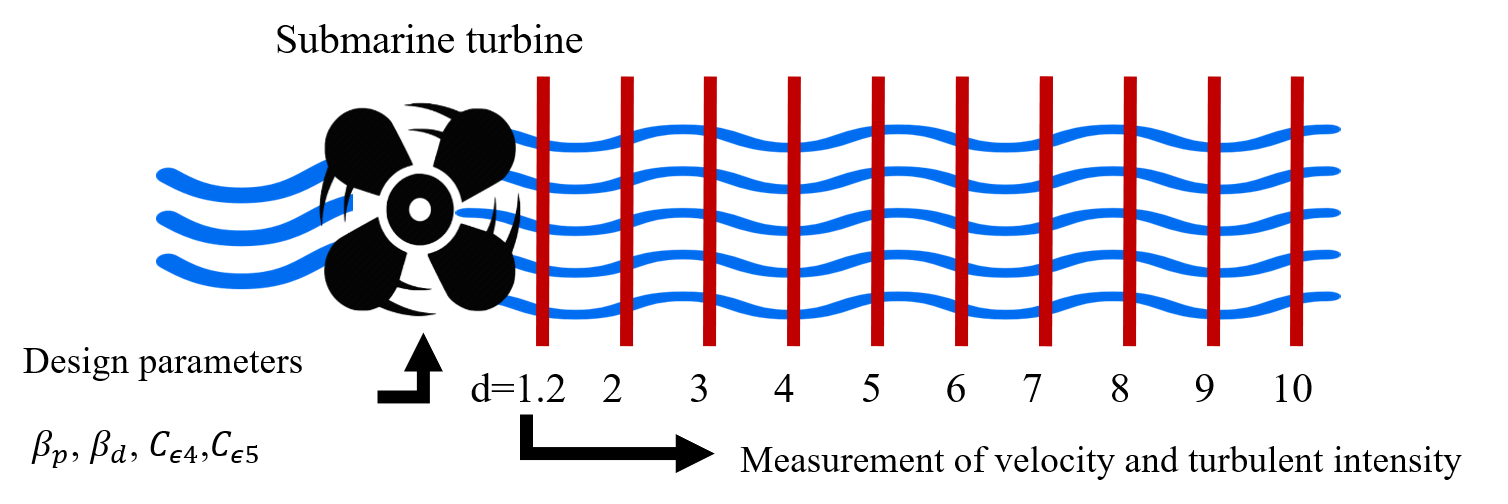
\includegraphics[width=1\textwidth]{images/marine.png}
	\caption{Marine Turbine's process}
	\label{fig:Marine Turbine}
\end{figure}

\chapter{Methodology}

This chapter contains four parts, including simulation, data preprocessing, surrogate model, and heuristic algorithm in Figure \ref{Flowchart for the surrogate-model framework}. We will introduce all of the following sections in details.

%To incorporate the surrogate model and metaheuristics into the problem of determining a set of unknown parameters in simulator, we should develop a standard in mathematical methodology to judge velocity and intensity of simulator with those parameters tuned by PSO and GA. Thus, we propose the following general procedure of the flowchart in offline optimization framework \ref{Flowchart for the surrogate-model framework}. 

\begin{figure}[h]
	\centering
	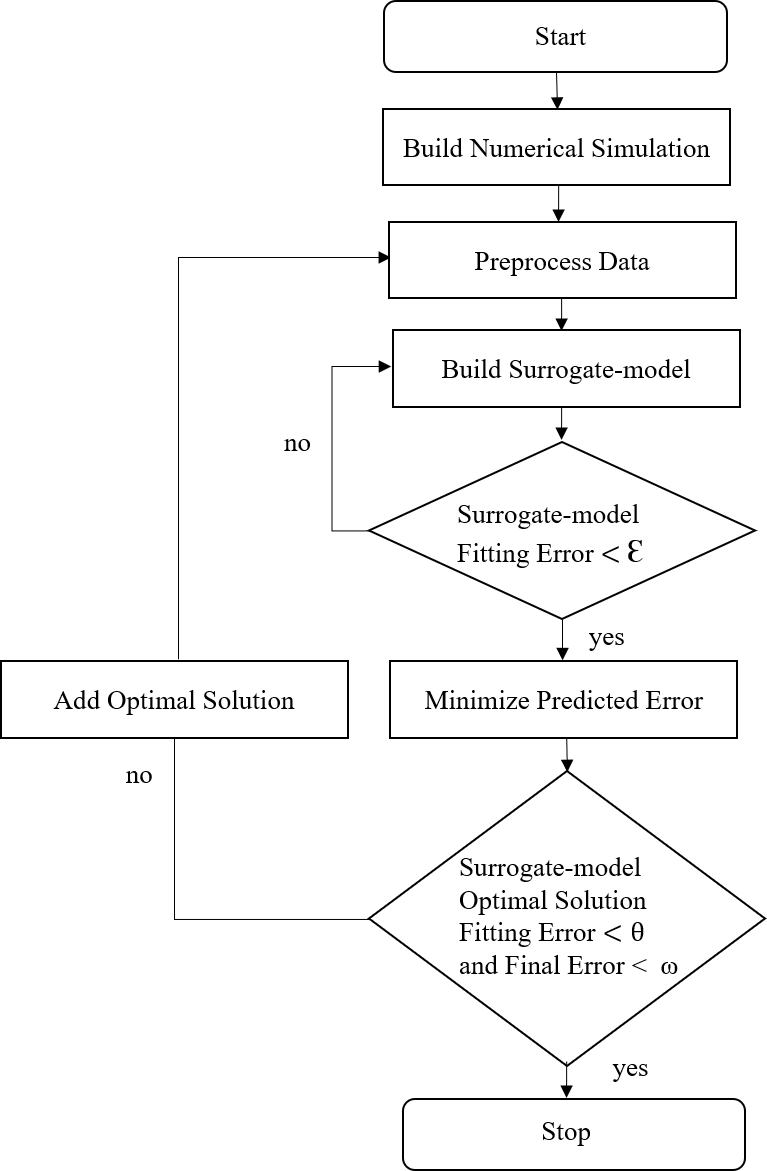
\includegraphics[width=0.5\textwidth]{images/flow.png}
	\caption{Flowchart for the surrogate-model framework. (Adapted from Sterling et al., 2019)}
	\label{Flowchart for the surrogate-model framework}
\end{figure}
\section{Simulation}
In our case, the simulator are used to predict the turbulence intensity ($I$) and velocity ($U$) each at two influent ${3\%}$ and ${15\%}$ which are written in $I_{3\%}$, $I_{15\%}$,$U_{3\%}$, and $U_{15\%}$ respectively. These quantities of interest (QoI) are all under ten different distance. Furthermore, we need to modify the simulation's parameters, so it is also important to define the design parameters of our simulator.
 
$\beta_{p}$, $\beta_{d}$, $C_{\epsilon4}$, $C_{\epsilon5}$ are the four parameters to be determined in the simulator. These parameters can come to the result of $y_{i,j,d}^S$. Then, $y_{i,j,d}^T$ is the physical experiment estimated by turbine marine. On the other hand, the surrogate model prediction noted as $\hat{y}_{i,j,d}$. All the variables are written in Table \ref{tab:definition variables}.

\begin{minipage}{\linewidth}
	%\centering
	\label{tab:definition variables} 
	\renewcommand\arraystretch{1}
	\captionof{table}{The definition of variables} 
	\begin{tabular}{lp{0.45\columnwidth}}
		\hline
		{\small Variable}     & {\small Definition}    \\
		\hline
		{\small $y_{i,j,d}^T$ $i$ = $3{\%}$, $15{\%}$ $j$ = $U$, $I$ $d$ = 1.2, 2, 3, 4, 5, 6, 7, 8, 9, 10}              &  
		$y_{i,j,d}^T$ is the state variables $j$ of physical experiment under the initial condition $i$ at spatial locations $d$.   \\
		{\small $y_{i,j,d}^S$ $i$ = $3{\%}$, $15{\%}$ $j$ = $U$, $I$ $d$ = 1.2, 2, 3, 4, 5, 6, 7, 8, 9, 10}              &  
		$y_{i,j,d}^S$ is the state variables $j$ of simulator prediction under the initial condition $i$ at spatial locations $d$.    \\
		{\small $\hat{y}_{i,j,d}$ $i$ = $3{\%}$, $15{\%}$ $j$ = $U$, $I$ $d$ = 1.2, 2, 3, 4, 5, 6, 7, 8, 9, 10}           & 
		$\hat{y}_{i,j,d}$ is the state variables $j$ of surrogate model's prediction under the initial condition $i$ at spatial locations $d$.\\
		{\small $\beta_{p}$} &
		The first parameter of the simulator.           \\
		{\small $\beta_{d}$}              &  
		The second parameter of the simulator.  \\
		{\small $C_{\epsilon4}$}              & 
		The third parameter of the simulator. \\
		{\small $C_{\epsilon5}$}              & 
		The fourth parameter of the simulator.  \\
		\hline
	\end{tabular}
\end{minipage}

\section{Data Preprocessing}

We will focus on the theory of clustering, outlier detection, and bootstrap that we have applied in the data preprocessing in this section.

\subsection{Clustering}
In the clustering, suppose that there is a set of d-dimensional data
\begin{equation}
x_{i}\in R^{d}, i=1,2,...,n
\end{equation}
Let K be the number of cluster which noted as {$S_{1}$, $S_{2}$,...,$S_{k}$}. The purpose of K-means clustering is to minimize the Euclidean distance of the number of data (n) and the center point in the group $x_{c}$. Then, $x_{i}$ will belong to the group which is the smallest Euclidean distance between it.The Euclidean equation is written in
\begin{equation}
arg\ min\sum_{c=1}^{K}\sum_{i=1}^{n}\left \| x_{i}- x_{c}\right \|^2
\end{equation}

\begin{figure}[h]
	\centering
	\subfigure[$x_{i}$ should be divided into two groups.]{
		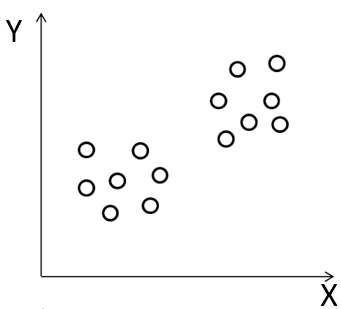
\includegraphics[width=5cm]{images/1C.PNG}
		%\caption{fig1}
	}
	\quad
	\subfigure[Define the center point of each group.]{
		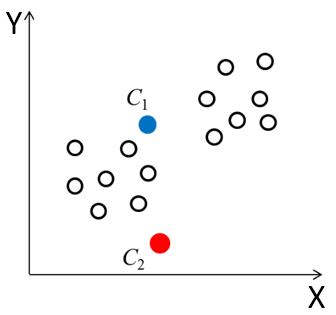
\includegraphics[width=5cm]{images/2C.PNG}
	}
	\quad
	\subfigure[Cause $d_{1}$<$d_{2}$, $x_{1}$ belongs to $C_{1}$.]{
		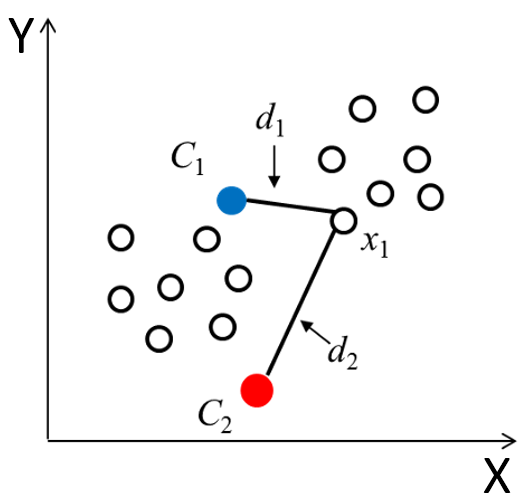
\includegraphics[width=5cm]{images/3C.PNG}
	}
	\quad
	\subfigure[Repeating (a) to (c) can finish grouping.]{
		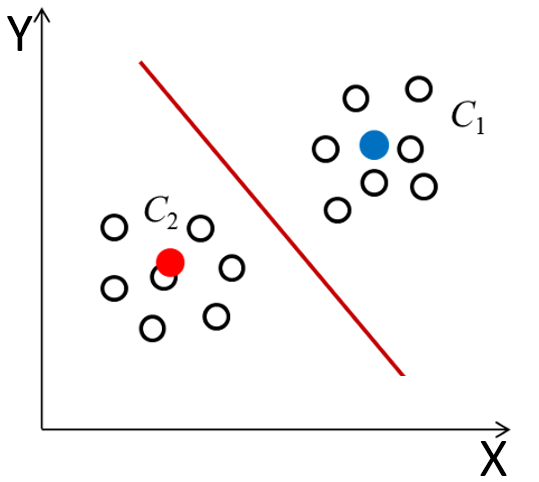
\includegraphics[width=5cm]{images/4C.PNG}
	}
	\caption{The concept of K-means clustering, adapted from http://medium.com/}
	\label{clusteringtheory}
\end{figure}
\subsection{Univariate Boxplot}
A univariate boxplot \cite{frigge1989some} is specified by five parameters: the two extremes, the upper UQ (75th percentile), lower LQ (25th percentile) quartiles, and the median (50th percentile). The lower and upper extremes of a boxplot are defined as

\begin{equation}
\label{eq:boxplot}
x_{L}=max\left \{ x_{(1)},LQ - \frac{3}{2} IQR\right \},
x_{U}=min\left \{ x_{(n)},UQ + \frac{3}{2} IQR\right \}.
\end{equation}

\begin{figure}[h]
	\centering
	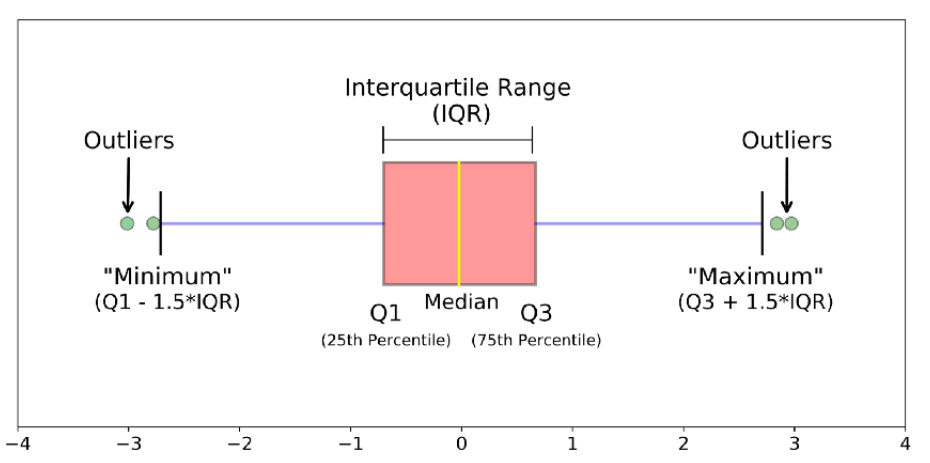
\includegraphics[width=1\textwidth]{images/boxplot.png}
	\caption{Different parts of a boxplot, adapted from http://towardsdatascience.com}
	\label{Boxplot}
\end{figure}
In Figure \ref{Boxplot} shows some outliers in the boxplot. We will remove the data that lays out of these two extremes.

\subsection{Bootstrap}

The basic idea of bootstrap or bootstrapping is that inference about a population from sample data can be modelled by resampling the sample data and performing inference about a sample from resampled data. In short, bootstrap resamples the data with replacement as illustrated in Figure 2.4. In bootstrap method, we keep resample the data in order to find the distribution of data. As we already know the data distribution, we only resample for the sufficient samples that we need in order to have enough datasets to train the model.  

\begin{figure}[h]
	\flushleft
	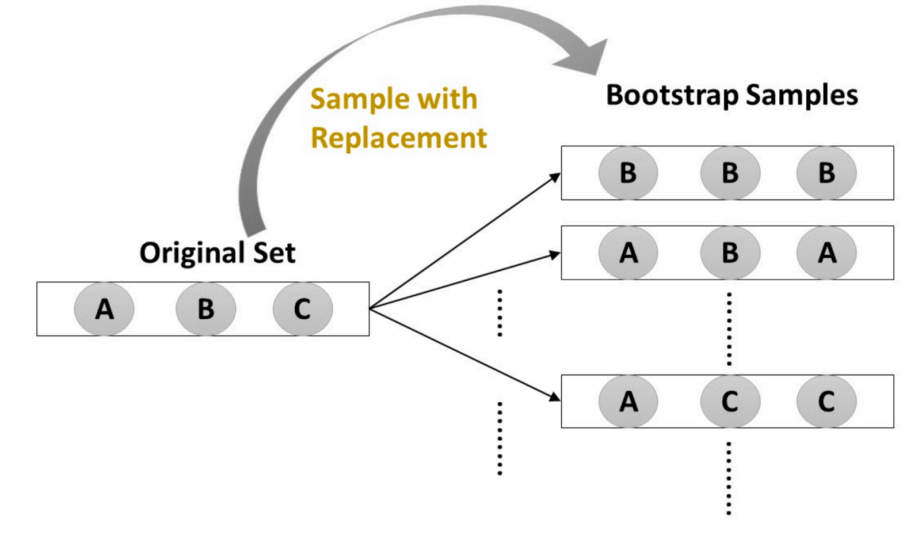
\includegraphics[width=1\textwidth]{images/bootstrap.png}
	\begin{flushright}
		\caption{Bootstrap, adapted from Chen (2019)}
	\end{flushright}
	\label{Bootstrap}
\end{figure}


\section{Surrogate Model}
In this section, we will introduce the selection of surrogate model, five-fold cross validation, and the Gaussian Process. 

\subsection{Selection of Surrogate Model}
The first time we get the data. It is difficult to know which is the best model to predict all these data. Luckily, scikit-learn, which is a library containing different kinds of package in the machine learning field, provides us with a cheat-sheet that illustrates four aspect of machine learning methodology such as regression, dimensionality reduction, clustering, and classification. In our case, regression is suitable for training the surrogate model. Now we have a set of regression model to be selected. It is necessary to define a quantitative measure, evaluating the error between the surrogate model predictions and numerical simulation. The mean absolute percentage error MAPE is chosen as a metric to compare surrogate model predictions with numerical simulation. In our paper, surrogate model fitting error MAPE$_{srgt/sim}$ is defined as 

\begin{equation}
\label{srgt/sim}
MAPE_{srgt/sim}=\frac{1}{N_{datasets}}\frac{1}{N_{points}}\sum_{m=1}^{\left | N_{datasets} \right |}\sum_{i}\sum_{d}\sum_{j}\left ( \frac{\left |\hat{y}_{i,j,d}-y_{i,j,d}^S \right |}{y_{i,j,d}^S} \right )
%MAPE_{srgt/sim}=\frac{1}{N_{datasets}}\frac{1}{\left | i \right|\left | d \right |\left | j \right |}\sum_{m=1}^{N_{datasets}}\sum_{i}\sum_{d}\sum_{j}\left ( \frac{\left |\hat{y}_{i,j,d}-y_{i,j,d}^S \right |}{y_{i,j,d}^S} \right )
\end{equation}

By choosing the smallest surrogate model fitting error MAPE$_{srgt/sim}$, we can make sure that this surrogate model can predict simulation's result well. 

\begin{figure}[h]
	\flushleft
	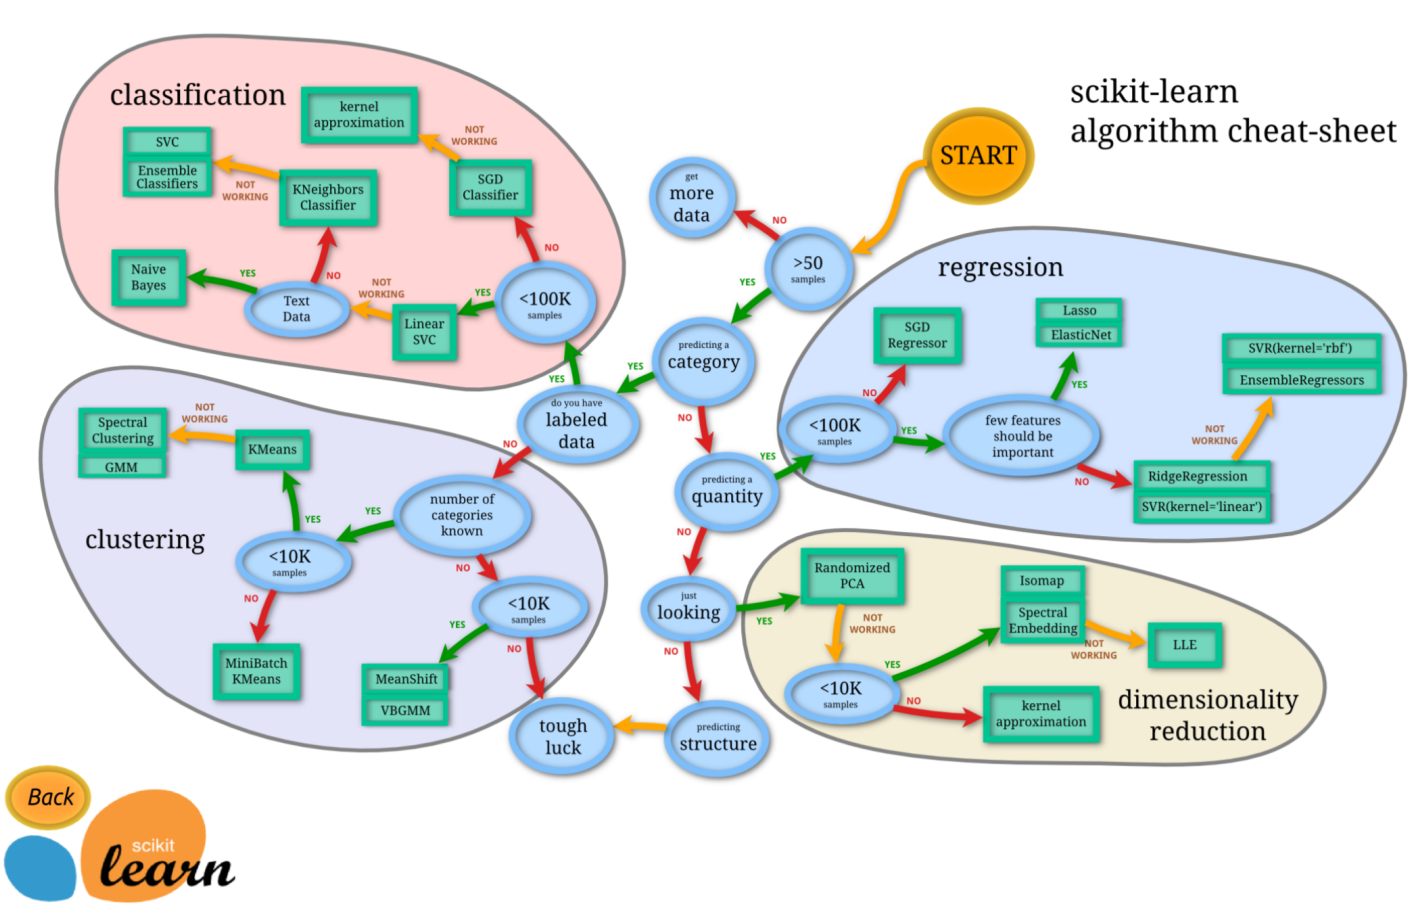
\includegraphics[width=1.15\textwidth]{images/scikit.png}
	\begin{flushleft}
		\caption{Mind map of machine learning, adapted from http://scikit-learn.org}
	\end{flushleft}
	\label{Mind map of machine learning}
\end{figure}

\subsection{K-fold cross-validation}

In order to avoid over-fitting, we often apply K-fold cross-validation. K is the number of group that we split. In Figure \ref{Five-fold cross-validation} is the example of five-fold cross-validation―that is, we split the training data into five sets, and we use each in turn as validation set to evaluate the model fit on the other four-fifths of the training set. Repeating the validation across different subsets gives us a better idea of the performance of the algorithm in advance. After doing five-fold cross-validation in training set, the surrogate model is built, and they should be tested. Therefore, testing set plays an important role to test whether the surrogate model is precise or not. 

\begin{figure}[h]
	\flushleft
	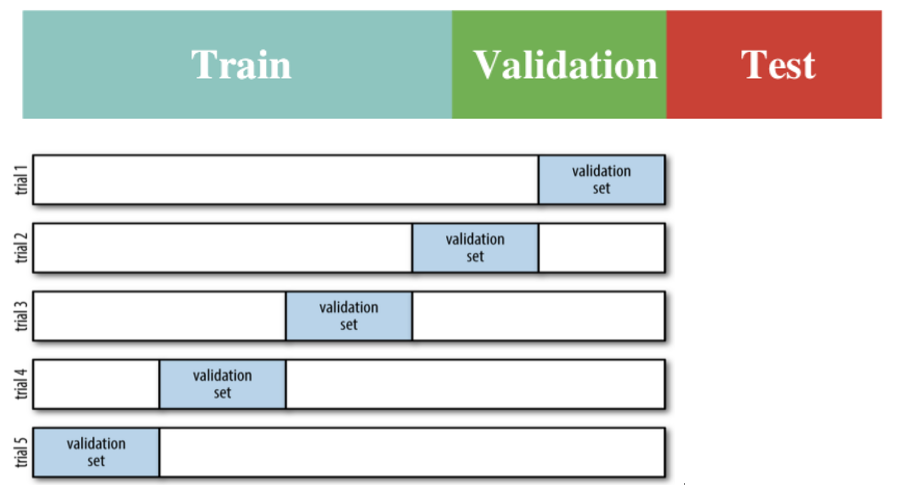
\includegraphics[width=1\textwidth]{images/5fold.png}
	\caption{Five-fold cross-validation, adapted from http://sebastianraschka.com}
	\label{Five-fold cross-validation}
\end{figure}

\subsection{Gaussian Process}

A Gaussian process is a collection of random variables, any finite set of which have a joint Gaussian distribution. A Gaussian process is completely specified by its mean function $m(x)$ and the covariance function $k(x,x′)$:

\begin{equation}
\label{mean function}
f({x})\sim GP(m({x}), k({x}, {x}^{\prime})). 
\end{equation}

There is a training set $D$ of n observations, $
D=\left \{ (x_{i},y_{i})\mid  i=1,…n \right \}
$ where x denotes an input vector like d, $\beta_{p}$, $\beta_{d}$, $C_{\epsilon4}$, $C_{\epsilon5}$ in our case, y denotes a scalar output or target such as $\hat{y}_{i,j,d}$ in this paper. The column vector inputs for all n cases are aggregated in the $D×n$ design matrix X and the targets are collected in the vector y.

The goal of Bayesian forecasting is to compute the distribution $p(y_{\ast}| x_{\ast} ,D)$ of output $y_{\ast}$  given a test input $x_{\ast}$ and a set of training points $D$. Using Bayesian rule, the posterior distribution for the Gaussian process outputs $y_{\ast}$ can be obtained. By conditioning on the observed targets in the training set, the predictive distribution is Gaussian:

\begin{equation}
\label{eq:gaussian distribution}
y_{\ast}\vert { x}_{\ast},{X},{y}\sim N(\hat{y}({ x}_{\ast}),\hat{\sigma}({ x}_{\ast})). 
\end{equation}
where, the mean and variance are given by
\begin{equation}
\label{eq:mean}
\qquad \ \ \hat{y}({x}_{\ast})={k}_{\ast}^{T}({ K}+\sigma_{n}^{2}{I})^{-1}{y}. 
\end{equation}
\begin{equation}
\label{eq:variance}
\hat{\sigma}({ x}_{\ast})= k({x}_{\ast},{x}_{\ast})-{ k}_{\ast}^{T}({ K}+\sigma_{n}^{2}{ I})^{-1}{ k}_{\ast}^{T}.
\end{equation}
where, a compact form of the notation setting for matrix of the covariance functions are: $k_{\ast}=K(X,x_{\ast})$, 
$K=K(X,X)$, $\sigma _{n}^{2}$ is the unknown variance of the Gaussian noise.
Gaussian process procedure can handle interesting models by simply using a covariance function with an exponential term:

\begin{equation}
\label{eq:exponential}
k_{y}(x_{p},x_{q})=\sigma_{f}^{2}\exp(-{1 \over 2l^{2}}(x_{p}-x_{q})^{2})+\sigma_{n}^{2}\delta_{pq}. 
\end{equation}

In addition to an exponential covariance function, there are five others in Table \ref{tab:covariance functions} 

\begin{minipage}{\linewidth}
	\centering
	\renewcommand\arraystretch{1.2}
	~\\
	\captionof{table}{The definition of covariance functions} \label{tab:covariance functions} 
	\begin{tabular}{lcc}
		\hline
		{\small Covariance function}     & {\small Equation}    \\
		\hline
		{\small ExpSineSquared}              &  $exp(-2(\frac{sin(\frac{\pi}{p}d(x_i, x_j))}{l})^2))$     \\
		{\small DotProduct}              &  $\sigma_{0}^{2}+x_i\cdot x_j$     \\
		{\small Radial-basis function(RBF)}           & 
		$exp(-\frac{1}{2} d(\frac{x_i}{l},\frac{x_j}{l})^2) $    \\
		{\small Rational quadratic(RQ)} &
		$(1+\frac{ d(x_i,x_j)^2 }{2\alpha l^2})^{-\alpha}$           \\
		{\small Matern}              &  $\frac{1}{2^{\upsilon -1}\Gamma \left ( \upsilon  \right )}\left ( \frac{\sqrt{2\upsilon }}{l}r \right )^{\upsilon }K_{\upsilon }\left ( \frac{\sqrt{2\upsilon }}{l}r \right )$    \\
		\hline
	\end{tabular}
\end{minipage}
~\\
Equation \ref{eq:exponential} expresses the idea the cases with nearby inputs will have highly correlated outputs. The covariance is denoted $k_{y}$ as it is for the noisy targets $y$ rather than for the underlying function $f$ GP employs a set of hyperparameters $\theta$ including the length-scale $l$, the signal variance $\sigma _{f}^{2}$and the noise variance $\sigma _{n}^{2}$, $\theta$ can be optimized based on log-likelihood framework:

\begin{equation}
\label{eq:likelihood}
\log p({y}\vert {X},{\theta})=  -{1 \over 2}{y}^{T}({K}+\sigma_{n}^{2}{I})^{-1}y-{1 \over 2}\log\vert {K}+\sigma_{n}^{2}{I}\vert -{n \over 2}\log 2\pi.
\end{equation}

Hyperparameters $\theta$  are initialized to random values (in a reasonable range) and then use an iterative method, for example conjugate gradient, to search for the optimal values.


\section{Metaheuristics}

In this section, we will provide two metaheuristics to minimize our predicted error.After building the suitable surrogate models, we should use metaheuristics to find the best parameters which can get lowest predicted error. In this paper, predicted error MAPE$_{srgt/exp}$ describes the difference between surrogate model prediction and physical experiment. The predicted error MAPE$_{srgt/exp}$ is written in

\begin{equation}
\label{srgt/exp}
%MAPE_{srgt/exp}=\frac{1}{40}\sum_{i}\sum_{d}\sum_{j}\left ( \frac{\left |\hat{y}_{i,j,d}-y_{i,j,d}^T \right |}{y_{i,j,d}^T} \right )
MAPE_{srgt/exp}=\frac{1}{N_{points}}\sum_{i}\sum_{d}\sum_{j}\left ( \frac{\left |\hat{y}_{i,j,d}-y_{i,j,d}^T \right |}{y_{i,j,d}^T} \right )
\end{equation}

The parameters predicted by metaheuristics will be set up in the simulator. After doing simulation, we will get $N_{points}$ of simulation result which will be verified with the surrogate model predictions. This optimal solution fitting error is also written in MAPE$_{srgt/sim}$. It is restricted to below $\theta$. If not, these $N_{points}$ points should be added as optimal solution points to the samples, and we should go to step two again in Figure \ref{Flowchart for the surrogate-model framework}. The optimal solution fitting error MAPE$_{srgt/sim}$ is formulated as

\begin{equation}
\label{optimal srgt/sim}
MAPE_{srgt/sim}=\frac{1}{N_{points}}\sum_{i}\sum_{d}\sum_{j}\left ( \frac{\left |\hat{y}_{i,j,d}-y_{i,j,d}^S \right |}{y_{i,j,d}^S} \right )
\end{equation}

The difference between $N_{points}$ of simulation result and the physical experiment is so called Final error MAPE$_{sim/exp}$. In our case, final error must be within $\omega$  because the smallest MAPE$_{sim/exp}$ of historical simulation data is $\omega$. We should find other parameters which are better than the historical ones; otherwise, the optimal solution points that we estimated will be added to the samples, and the surrogate model should be rebuilt. The final error MAPE$_{sim/exp}$ is the form of

\begin{equation}
\label{final sim/exp}
MAPE_{sim/exp}=\frac{1}{N_{points}}\sum_{i}\sum_{d}\sum_{j}\left ( \frac{\left |y_{i,j,d}^S-y_{i,j,d}^T \right |}{y_{i,j,d}^T} \right )
\end{equation}

\subsection{Genetic Algorithm}

Genetic Algorithm (GA) is a metaheuristic search algorithm based on the
evolutionary. The main idea is derived from the behavior of reproduction animal which consists of selection, crossover and mutation. GA represent an intelligent exploitation of a random search. It has been applied to solve optimization problem for many years. The original Genetic Algorithm consists of the following component as Figure \ref{Flowchart for implementation of genetic algorithm}. First, we should generate the initial population. If the chromosome has $N_{var}$ variables (an $N_{var}$-dimensional optimization problem) given by P1, P2,..., P($t$) , then the chromosome is written as an $N_{var}$ element row vector.
\begin{equation}
chromosome = [P_{1},P_{2},P_{3},…,P_{N_{var}}]
\end{equation}
In our case, we generate some sets of initial populations of chromosome = [$P_{\beta_{p}}$,$P_{\beta_{d}}$, $P_{C_{\epsilon4}}$, $P_{C_{\epsilon5}}$] randomly. Then, we define the fitness function of the populations as

\begin{equation}
\label{gasrgt/exp}
\min MAPE_{srgt/exp}=\frac{1}{N_{points}}\sum_{i}\sum_{d}\sum_{j}\left ( \frac{\left |G(\beta_{p}, \beta_{d}, C_{\epsilon4}, C_{\epsilon5})-y_{i,j,d}^T \right |}{y_{i,j,d}^T} \right )
\end{equation}

Each set of fitness function will be evaluated. Because we want to get the
smallest fitness function by counting down the fitness function. Let a set of variables with the smallest fitness function is prone to be selected by Roulette wheel selection. Next step is doing encoding which can make the chromosome be binary variable in Figure \ref{decode}. As binary code length(n) is defined, the range of upperbound $\bar{x}$ and lowerbound $\underline{x}$ can be divided into $2^{n}$. After we match the variable values to binary variable, the genes can apply one-point crossover operator to obtain a child chromosome C($t$) like C1 and C2. Then, we can also apply mutation operator to C1 and C2 with mutation rate Pm($t$) to produce D($t$) as a child after mutation. Finally, we evaluate chromosome $P_{N_{var}}$, C1, C2, D($t$) by decoding these binary variables into value and count their fitness ranking to have the best set of $\beta_{p}$, $\beta_{d}$, $C_{\epsilon4}$, $C_{\epsilon5}$ as our solution. At the end, if GA reach the maximum stopping criteria then stop; otherwise, return to Step 1.

\begin{figure}[h]
	\centering
	
\includegraphics[width=0.5\textwidth]{images/chromosome.png}
	\caption{Four continuous parameter values are graphed with the quantization levels shown. The corresponding gene or chromosome indicates the quantization level where the parameter value falls.This figure adapted from \cite{haupt2004practical}}
	\label{decode}
\end{figure}


\begin{figure}[h]
	\centering
	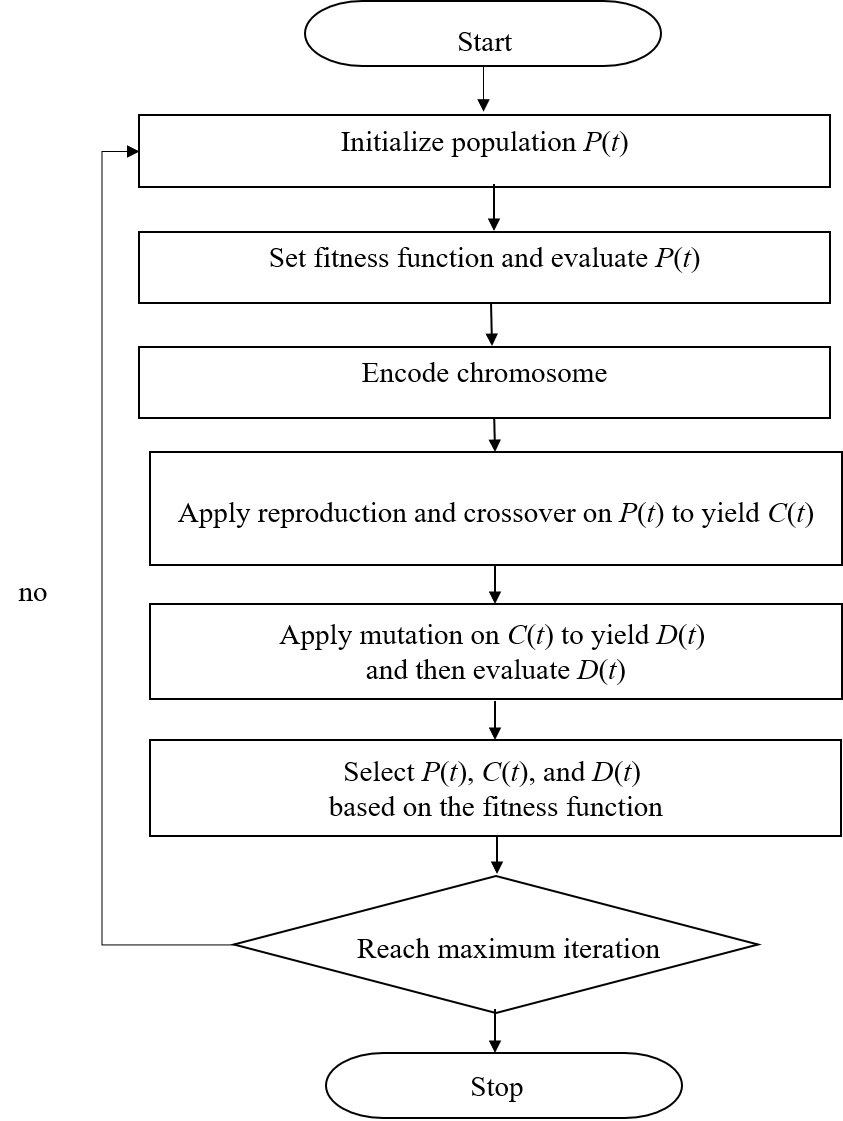
\includegraphics[width=0.48\textwidth]{images/GA.png}
	\caption{Flowchart for implementation of Genetic Algorithm}
	\label{Flowchart for implementation of genetic algorithm}
\end{figure}

\subsection{Particle Swarm Optimization Algorithm}

PSO is initialized with a population of random solutions and searches for optima by updating generations. In PSO, the potential solutions, called particles, fly through the problem space by following the current optimum particles. Each particle keeps track of its coordinates in the problem space which are associated with the best solution it has achieved so far. This value is called $p_{best}$. Another “best” value that is tracked by the particle swarm optimizer is the best value, obtained so far by any particle in the neighbors of the particle. When a particle takes all the population as its topological neighbors, the best value is a global best and is called $g_{best}$. After finding the two best values, the particle updates its velocity and positions with following equation:

\begin{equation}
\label{eq:PSO}
\left.\matrix{v_{id}^{t}=v_{id}^{t-1}+c_{1}r_{1}(p_{id}-x_{id}^{t-1})+c_{2}r_{2}(p_{gd}-x_{id}^{t-1})\cr x_{id}^{t}=x_{id}^{t-1}+v_{id}^{t}\hfill}\right \} 
\end{equation}

$v_{id}^{t-1}$ is velocity of the $i^{th}$ particle in $d$ dimension space at the time of $t-1$; $x_{id}^{t-1}$ is location of the $i^{th}$ particle at the $d$ dimensions at the time of $t-1$; $r_{1}$ and $r_{2}$ are random number distributed uniformly in (0,1). $c_{1}$ and $c_{2}$ are learning factors; $p_{id}$ is $p_{best}$ and $p_{gd}$ is $g_{best}$. As Figure \ref{Flowchart for implementation of particle swarm optimization} shows, each particle represents a set of $\beta_{p}$, $\beta_{d}$, $C_{\epsilon4}$, $C_{\epsilon5}$ in our paper. The second step is that we will evaluate the fitness of each particle by Equation \ref {srgt/exp}. Then, the particles will also update their positions by the randomizer $r_{t}$ and learning rate $c_{t}$ to modify their local best $p_{gd}$ and global best $ p_{gd} $. $p_{gd}$ is the solution of Equation \ref {srgt/exp}. $p_{gd}$ with the minimum solution of Equation \ref {srgt/exp} has the best set of parameters. If PSO reach the maximum stopping criteria then stop; otherwise, return to Step 2. 

\begin{figure}[h]
	\centering
	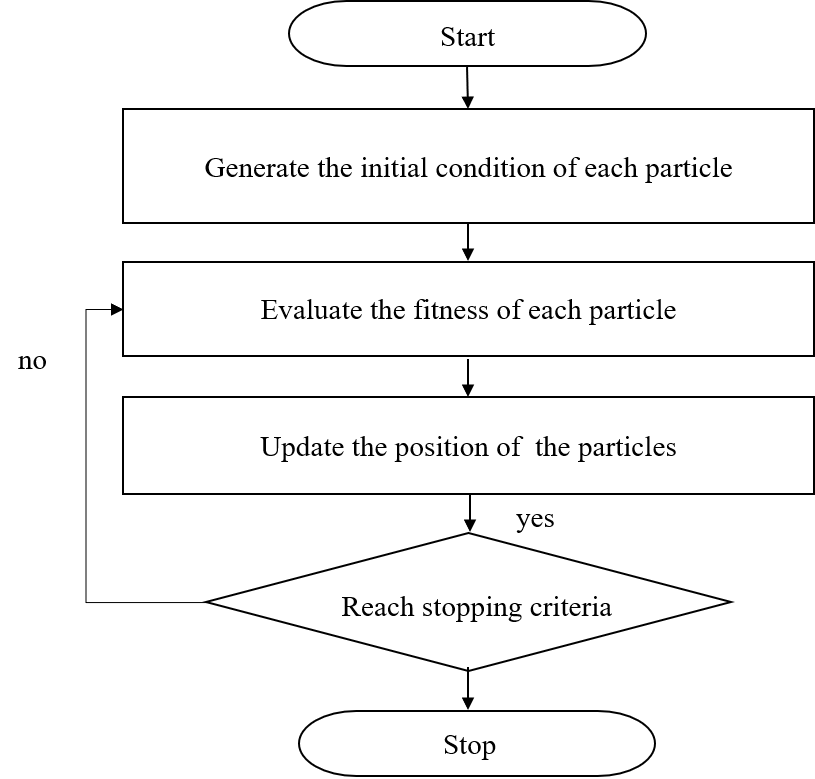
\includegraphics[width=0.8\textwidth]{images/PSO.png}
	\caption{Flowchart for implementation of Particle Swarm Optimization }
	\label{Flowchart for implementation of particle swarm optimization}
\end{figure}


\chapter{Numerical Analysis}

\section{Data Intergration}
According to the physical experiment of Sandia National Laboratories (SNL), there is a set of state variables under ten different spatial distances. Instead of doing physical experiment, which is quite repetitive, time-consuming, expensive and environmentally damaging, we apply computer simulator and surrogate model to predict the result of the physical experiment under different parameters. However, some of the data which are generated from the simulator are not as moderate as our thought, so we should do data preprocessing to enhance the accuracy of the prediction. Figure \ref{fig:clustering} shows the distribution of the physical experiment and simulation, namely numerical experiments before data preprocessing.


\begin{figure}[htbp]
\centering
\subfigure[The distribution of $I_{3{\%}}$ experiment.]{
	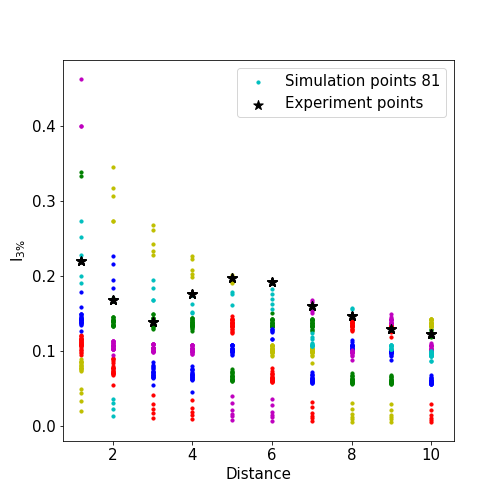
\includegraphics[width=7cm]{images/TI03.png}
	%\caption{fig1}
}
\quad
\subfigure[The distribution of $I_{15{\%}}$ experiment.]{
	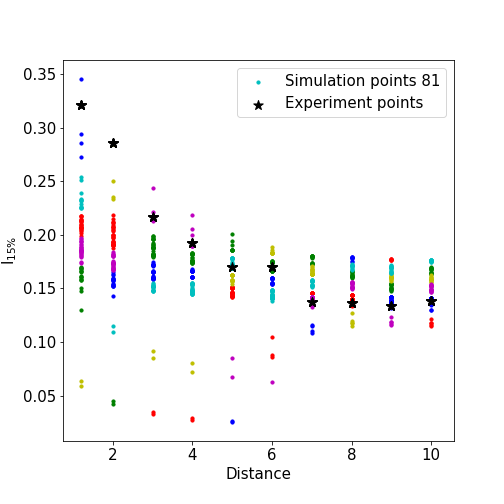
\includegraphics[width=7cm]{images/TI15.png}
}
\quad
\subfigure[The distribution of $U_{3{\%}}$ experiment.]{
	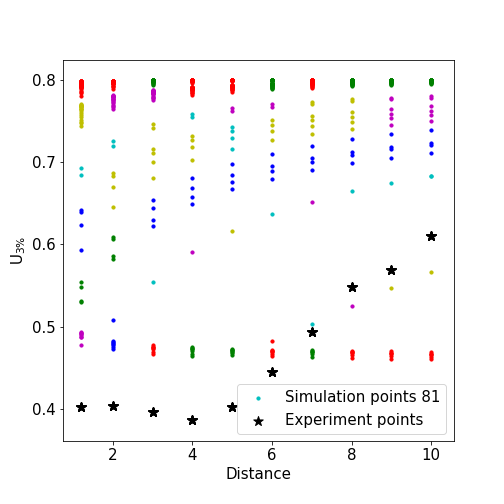
\includegraphics[width=7cm]{images/U03.png}
}
\quad
\subfigure[The distribution of $U_{15\%}$ experiment.]{
	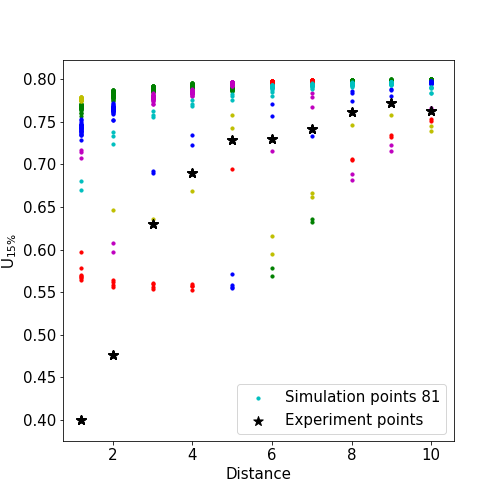
\includegraphics[width=7cm]{images/U15.png}
}
\caption{The distribution of the physical experiment and the numerical experiment.}
\label{fig:clustering}
\end{figure}

As Figure \ref{fig:clustering} shows, the horizontal axis represents ten distance points, while the state variables $U_{3{\%}}$, $U_{15{\%}}$, $I_{3{\%}}$, $I_{15{\%}}$ are presented in the vertical axis of each sub-graph individually. We apply K-means clustering to the data under different distances by dividing them into six groups. By applying K-means clustering, we set cluster number into 6 and random state number as 42. The group which is the closest to the physical experimental points (marked with black pentagram) is chosen, and our new set of data will be extracted from them. 

In order to avoid over-fitting, the whole datasets should be divided into 70{\%} of training set and 30{\%} of testing set. Training set is used to build the surrogate model, and testing set is to verify the accuracy of the model. In this paper, the number of 97 datasets are separated into 81 datasets for training and 16 datasets for testing. After K-means clustering, we reduce 81 datasets to 36 datasets and retrieve them to be our surrogate model training dataset.

\begin{figure}[htbp]
	\centering
	\subfigure[The boxplot distribution of $I_{3{\%}}$ experiment.]{
		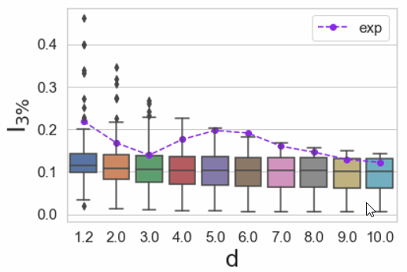
\includegraphics[width=7cm]{images/pic_I03.png}
		%\caption{fig1}
	}
	\quad
	\subfigure[The boxplot distribution of $I_{15{\%}}$ experiment.]{
		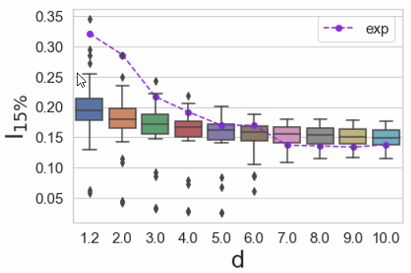
\includegraphics[width=7cm]{images/pic_I15.png}
	}
	\quad
	\subfigure[The boxplot distribution of $U_{3{\%}}$ experiment.]{
		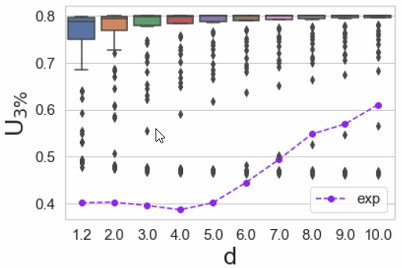
\includegraphics[width=7cm]{images/pic_U03.png}
	}
	\quad
	\subfigure[The boxplot distribution of $U_{15\%}$ experiment.]{
		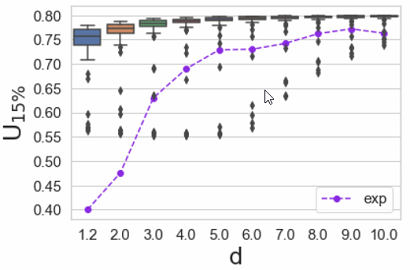
\includegraphics[width=7cm]{images/pic_U15.png}
	}
	\caption{The boxplot distribution of the physical experiment and the numerical experiment without clustering.}
	\label{fig:noclustering}
\end{figure}

\begin{figure}[htbp]
	\centering
	\subfigure[The boxplot distribution of $I_{3{\%}}$ experiment.]{
		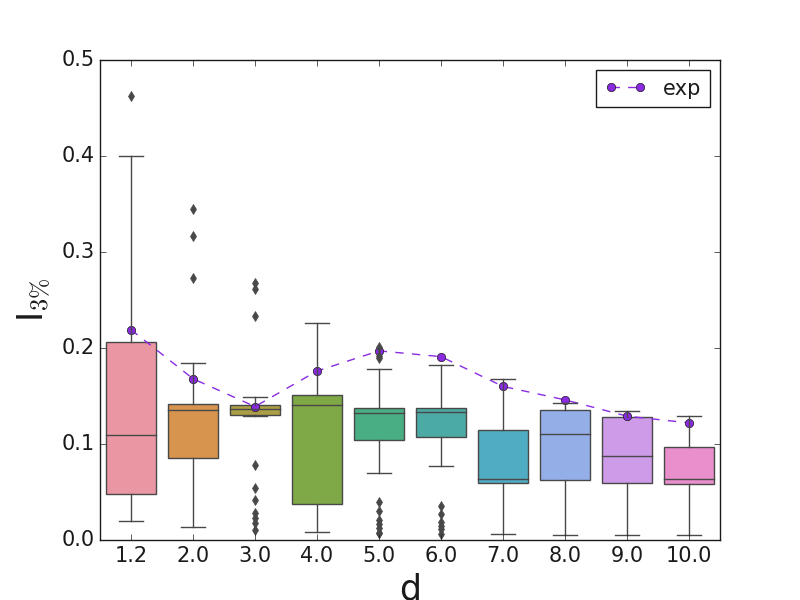
\includegraphics[width=7cm]{images/cluster_ti03.PNG}
		%\caption{fig1}
	}
	\quad
	\subfigure[The boxplot distribution of $I_{15{\%}}$ experiment.]{
		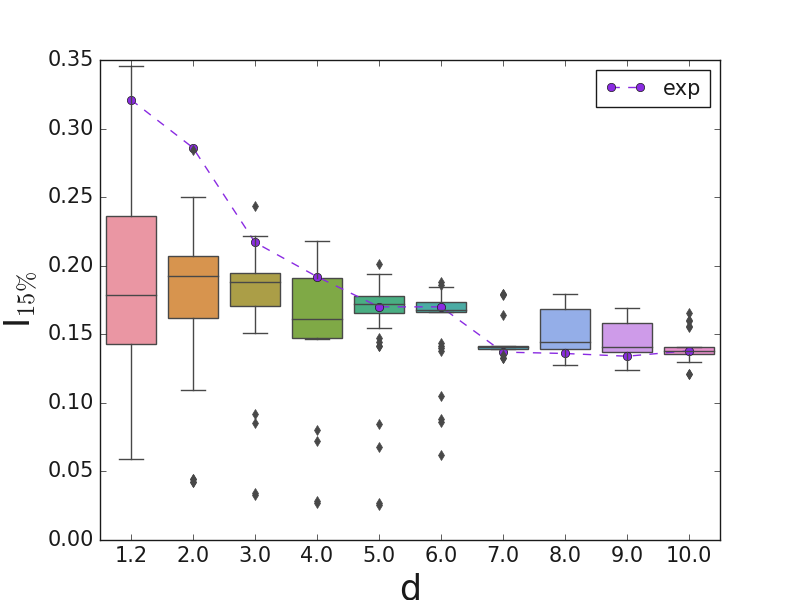
\includegraphics[width=7cm]{images/cluster_ti15.PNG}
	}
	\quad
	\subfigure[The boxplot distribution of $U_{3{\%}}$ experiment.]{
		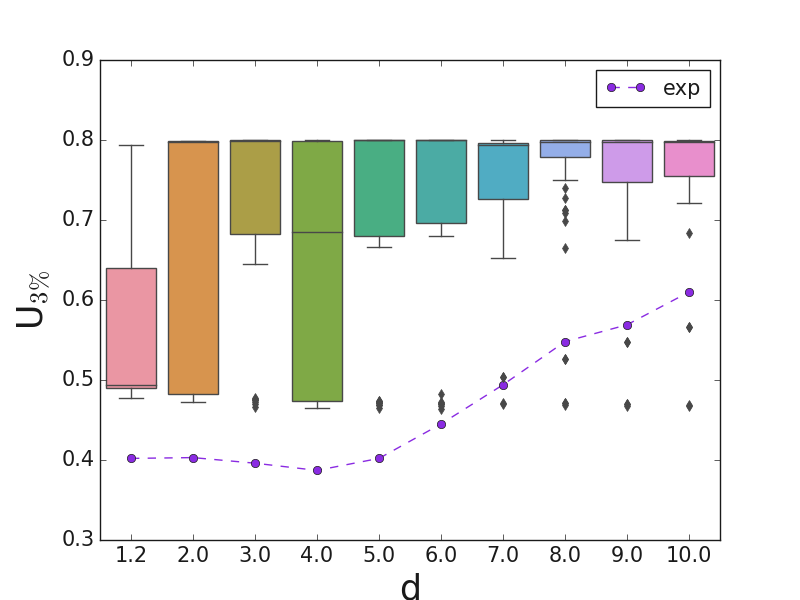
\includegraphics[width=7cm]{images/cluster_vel03.PNG}
	}
	\quad
	\subfigure[The boxplot distribution of $U_{15\%}$ experiment.]{
		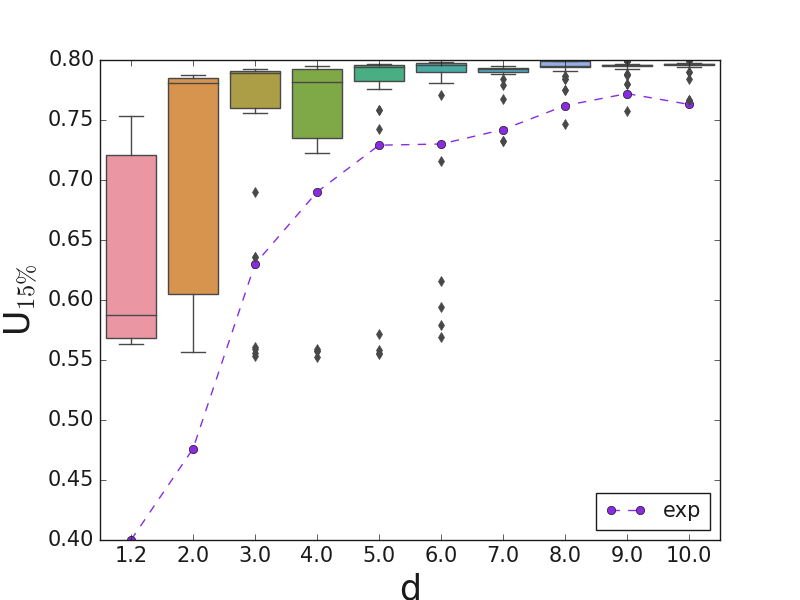
\includegraphics[width=7cm]{images/cluster_vel15.PNG}
	}
	\caption{The boxplot distribution of the physical experiment and the numerical experiment with clustering.}
	\label{fig:withclustering}
\end{figure}

In this section, we will also compare the Figure \ref{fig:noclustering} with Figure \ref{fig:withclustering} to show the data distribution after clustering. Also, Figure \ref{fig:noclustering} is in comparison to Figure \ref{fig:withoutlier} to present the data distribution after applying outlier detection.Finally, we will compare Figure \ref{fig:withclustering} with Figure \ref{fig:withbootstrap} to verify that there is no change on data distribution after using bootstrap method. We use these four kinds of boxplot to verify each data preprocessing which has the positive effect on surrogate model's prediction.

Figure \ref{fig:noclustering} represents 81 datasets without any data preprocessing, whereas Figure \ref{fig:withclustering} shows these datasets with clustering. After applying clustering, the historical experiment of $U_{3{\%}}$ and $U_{15{\%}}$ gets closer to the physical experiment. Therefore, it is necessary to apply this method. 

As Figure \ref{fig:outlier a} shows, the retrieved dataset doesn't obey Gaussian distribution so it is necessary to use univariate boxplot in order to remove the outliers \cite{shevlyakov2013robust}. By applying outlier detection, we set a function called detect outliers which contains the calculation of  LQ(25th percentile), median(50th percentile), UQ(75th percentile),
IQR(Interquartile range), $x_{L}$(minimum), and $x_{U}$(maximum). If the point , which is below the range of $x_{L}$ and above the range of $x_{U}$, will be regarded as outlier, so we will remove all of them.

As Figure \ref{fig:withoutlier} shows, we have removed most of the outlier points by comparing with Figure \ref{fig:noclustering}. But once the points have been removed the UQ, LQ, median and two extremes will be changed. It is difficult to retrieve all the points that are between $x_{L}$ and $x_{U}$ so now we still have some outlier points in $U_{3{\%}}$, $U_{15{\%}}$, $I_{3{\%}}$, and $I_{15{\%}}$.

\begin{figure}[htbp]
	\centering
	\subfigure[Distribution of state variables with outliers.]{
		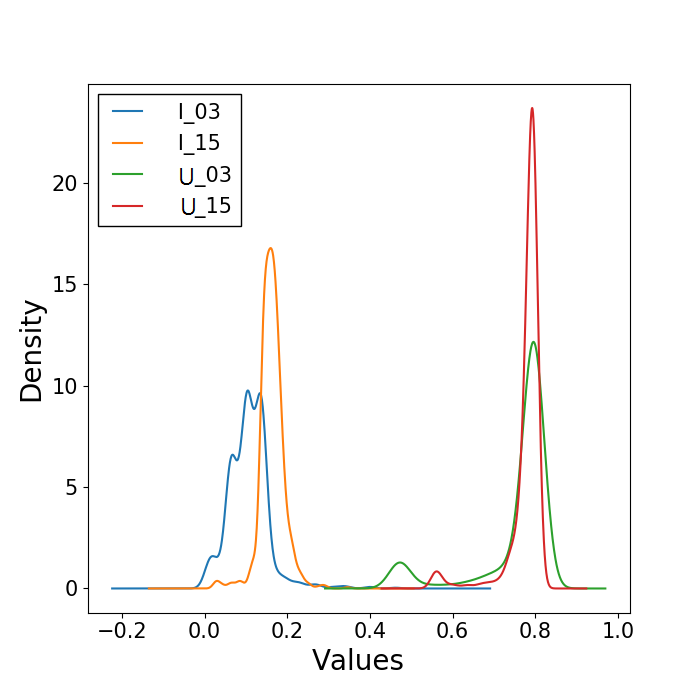
\includegraphics[width=7cm]{images/BG.png}
		%\caption{fig1}
		\label{fig:outlier a}
	}
	\quad
	\subfigure[Distribution of state variables without outliers.]{
		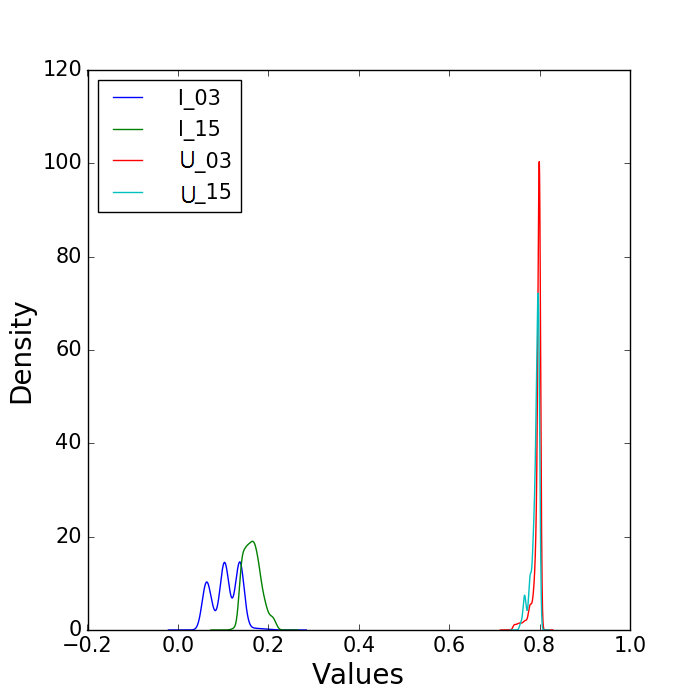
\includegraphics[width=7cm]{images/AG.png}
		\label{fig:outlier b}
	}
\caption{Using boxplot to remove the outliers}
\label{fig:outlier}
\end{figure}

\begin{figure}[htbp]
	\centering
	\subfigure[The distribution of $I_{3{\%}}$ experiment.]{
		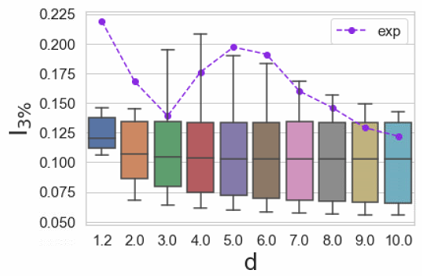
\includegraphics[width=7cm]{images/outlier_I03.png}
		%\caption{fig1}
	}
	\quad
	\subfigure[The distribution of $I_{15{\%}}$ experiment.]{
		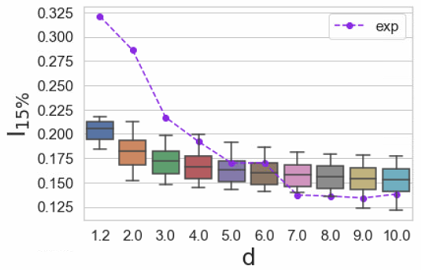
\includegraphics[width=7cm]{images/outlier_I15.png}
	}
	\quad
	\subfigure[The distribution of $U_{3{\%}}$ experiment.]{
		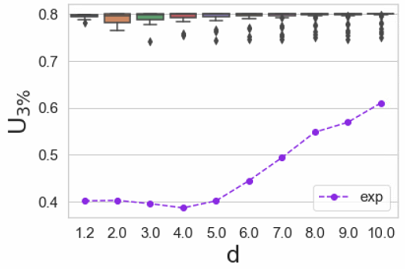
\includegraphics[width=7cm]{images/outlier_U03.png}
	}
	\quad
	\subfigure[The distribution of $U_{15\%}$ experiment.]{
		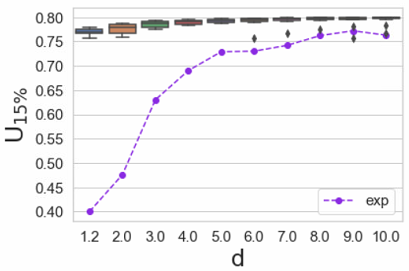
\includegraphics[width=7cm]{images/outlier_U15.png}
	}
	\caption{The distribution of the physical experiment and the numerical experiment with outlier.}
	\label{fig:withoutlier}
\end{figure}

\begin{figure}[htbp]
	\centering
	\subfigure[The distribution of $I_{3{\%}}$ experiment.]{
		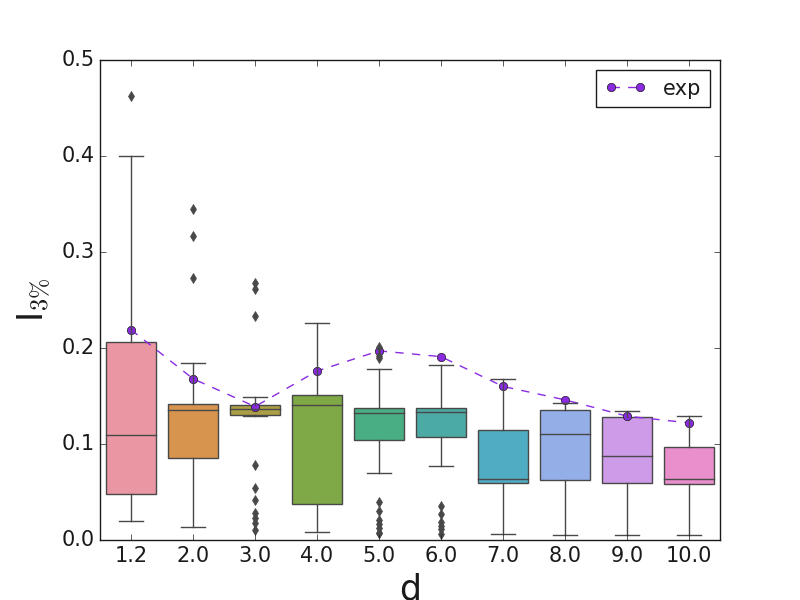
\includegraphics[width=7cm]{images/bootstrap_I03.png}
		%\caption{fig1}
	}
	\quad
	\subfigure[The distribution of $I_{15{\%}}$ experiment.]{
		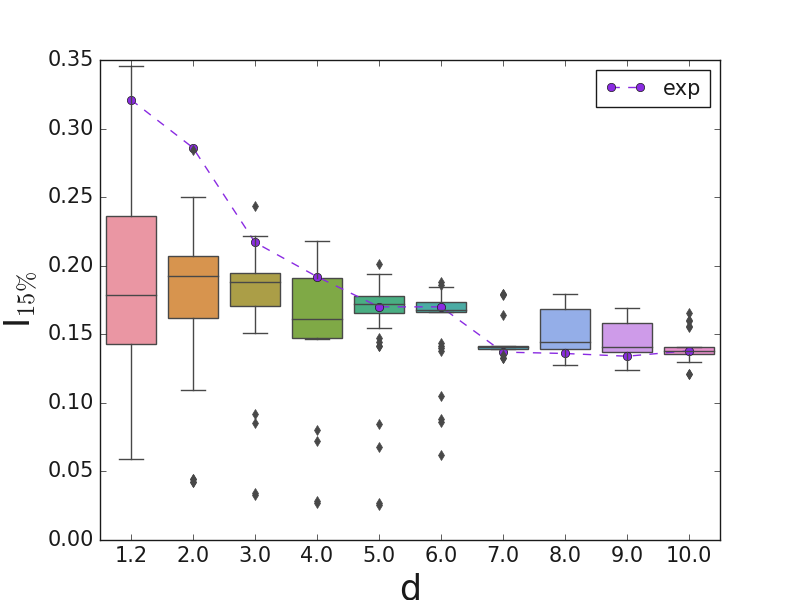
\includegraphics[width=7cm]{images/bootstrap_I15.png}
	}
	\quad
	\subfigure[The distribution of $U_{3{\%}}$ experiment.]{
		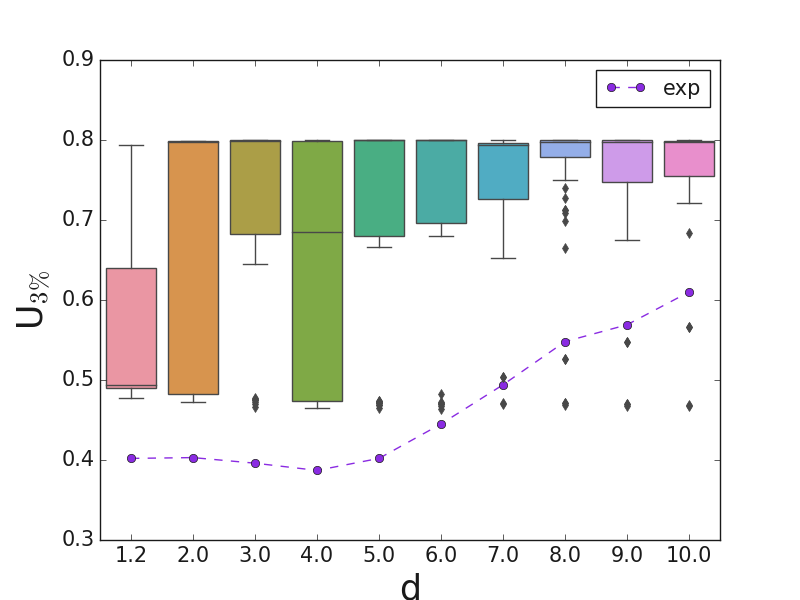
\includegraphics[width=7cm]{images/bootstrap_U03.png}
	}
	\quad
	\subfigure[The distribution of $U_{15\%}$ experiment.]{
		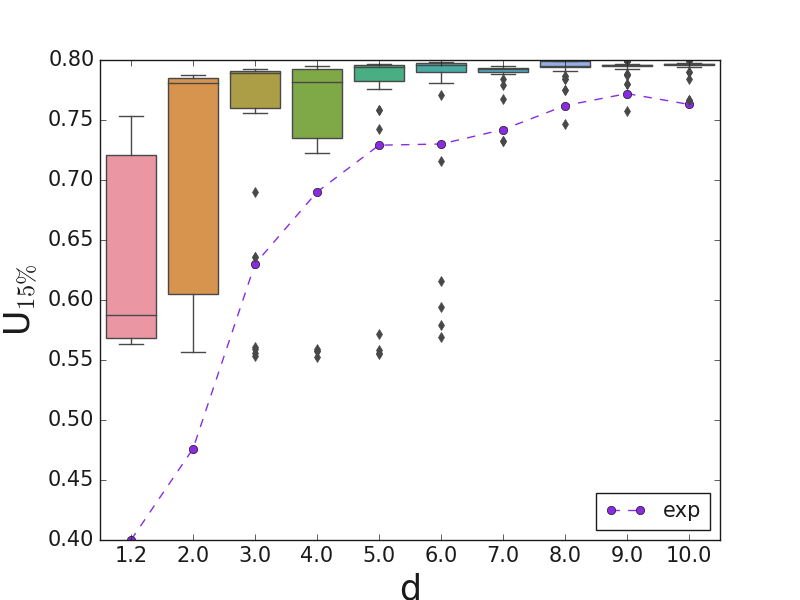
\includegraphics[width=7cm]{images/bootstrap_U15.png}
	}
	\caption{The distribution of the physical experiment and the numerical experiment with bootstrap.}
	\label{fig:withbootstrap}
\end{figure}

Besides, we use bootstrap method that involves iteratively resampling the 27 datasets with replacement. We use for loop to randomly select the 270 points for 1000 times and finally get 100 datasets. After this method, we increase the number of datasets into 100 datasets. Because all of the dataset are based on the original one, Figure \ref{fig:withbootstrap} is the same as Figure \ref{fig:withclustering}. After these data preprocessing, it is about to train our model with 100 datasets. 

\section{Surrogate Model Development}
In this section, we will use Equation \ref{srgt/sim} as the evaluative criteria to evaluate the performance of the surrogate model. By following Figure 2.5, the samples in our research are only 810 points which are less than the number of 100K so it is reasonable to use Lasso, ElasticNet, SVR, RidgeRegression and EnsembleRegressors to build the surrogate model.

\begin{flushleft}
\begin{figure}[h]
	\flushleft
	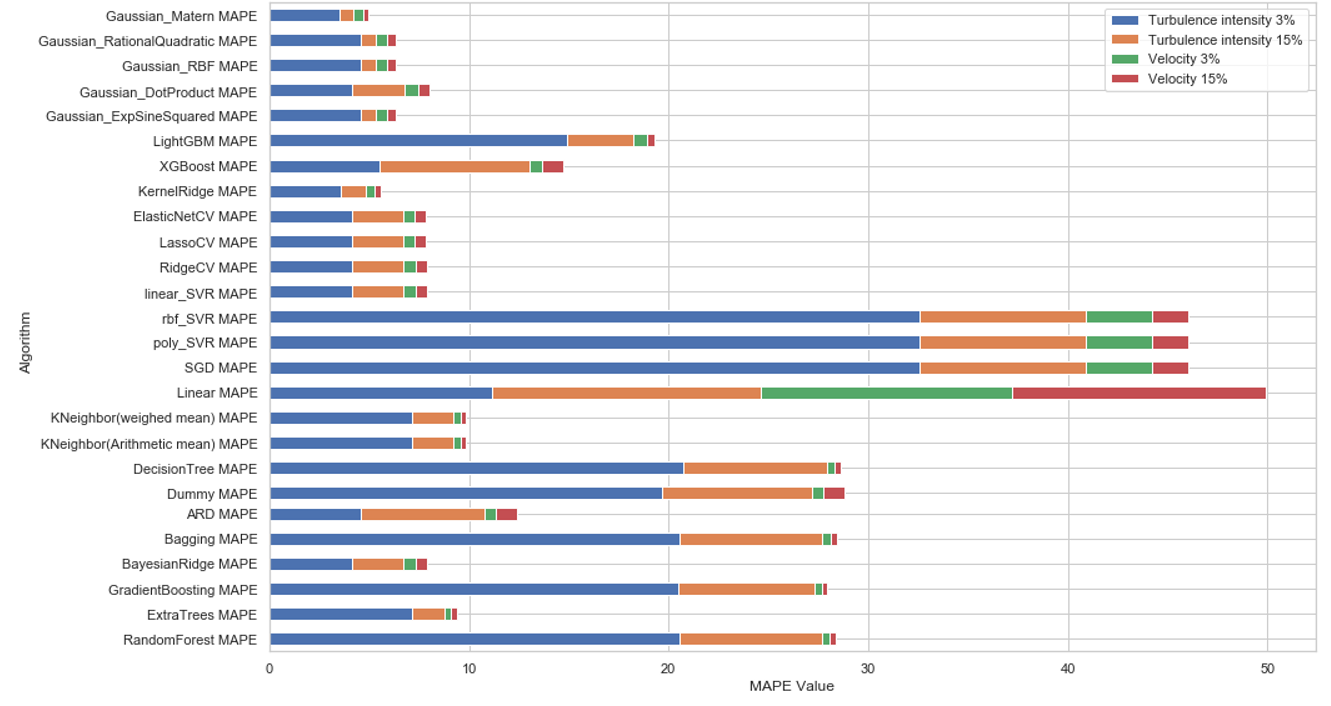
\includegraphics[width=1.2\textwidth]{images/regr.png}
	\begin{flushright}
		\caption{The MAPE of different kinds of machine learning regression}
	\end{flushright}
	\label{fig:MAPEregression}
\end{figure}
\end{flushleft}

The Figure 3.4 presents information about the total percentage of MAPE in $U_{3{\%}}$, $U_{15{\%}}$, $I_{3{\%}}$ and $I_{15{\%}}$ predicted by different machine learning models. 

Before the data is analyzed, it is difficult to know which is the best one from these twenty-six models. Through trial and error method, Gaussian model with five kinds of different kernel functions is the fittest, compared with three types of Support Vector Regression (SVR), Lasso and Ridge Regression, Decision tree and so on. All the total MAPE values of Gaussian models are under $\epsilon$ = ${10{\%}}$. $U_{3{\%}}$ always takes the lowest percentage within these four state variables. 

Overall, the Gaussian model is noticeably lower in the MAPE of $U_{3{\%}}$, $U_{15{\%}}$, $I_{3{\%}}$ and $I_{15{\%}}$, so the whole dataset will be trained by this model.

\section{Building Gaussian Process Regression}

The training set, which contains 100 datasets and is close to the physical experimental points, is about to build Gaussian model. 

The Gaussian Process Regression (GPR) surrogate model is constructed using Python version 3.6.4 with Numpy version 1.14.3 and Pandas version 0.22.0. The GPR is trained by scikit-learn 0.19.1, and the graph is drawn by Matplotlib version 2.1.2. The processor is GPU GeForce GTX 1060 which is extremely faster than the traditional computer equipped with CPU.

The GPR model is trained to minimize the fitting error between the surrogate model and simulator by adjusting kernel and alpha. The kernel with the lowest MAPE should be found by testing one by one. In contrast, alpha can be precisely predicted by grid search method which is tuned in the range $10^{-5}$ to $10^{5}$. Table \ref{tab:Summary of the covariance functions} shows five different kernels of GPR in $U_{3{\%}}$, $U_{15{\%}}$, and $I_{15{\%}}$ with alpha 0.00001 and the remaining $I_{3{\%}}$ with alpha 0.0001.

Surrogate-model fitting error MAPE$_{srgt⁄sim}$ Equation \ref{srgt/sim} is an indicator of the performance in five kernels. All the MAPE$_{srgt⁄sim}$ values are estimated by five-fold cross-validation in Figure \ref{Five-fold cross-validation}. After doing five-fold cross-validation in training set, the GPR model is built, and it need to be tested. Therefore, testing set $N_{datasets}$ = 16 will test whether the GPR model is precise or not. 

\begin{minipage}{\linewidth}
	\centering
	\renewcommand\arraystretch{1}
	~\\
	\captionof{table}{Summary of the covariance functions} \label{tab:Summary of the covariance functions} 
	\begin{tabular}{lccccc}
		\hline
		{\small QoI} & {\small ExpSineSquared} & {\small DotProduct} & {\small RBF} & {\small RQ} & {\small Matern}\\
		\hline
		{\small $U_{3{\%}}$}              &  
		5.6${\%}$ & 3.2${\%}$ & 5.6${\%}$ & 5.6${\%}$ & 2.5${\%}$   \\
		{\small $U_{15{\%}}$}              &  
		0.6${\%}$ & 0.6${\%}$ & 0.6${\%}$ & 0.5${\%}$ & 0.6${\%}$     \\
		{\small $I_{3{\%}}$}           & 
		18.8${\%}$ & 14.3${\%}$ &18.8${\%}$ & 18.8${\%}$ & 15.9${\%}$   \\
		{\small $I_{15{\%}}$} &
		1.2${\%}$ & 2.8${\%}$ &1.2${\%}$ & 1.2${\%}$ & 1.2${\%}$           \\
		\hline
		{\small Mean}              &  
		6.55${\%}$ & 5.2${\%}$ & 6.55${\%}$ & 6.5${\%}$ & 5${\%}$     \\
		\hline
	\end{tabular}
\end{minipage}

Table \ref{tab:Summary of the covariance functions} presents the result of testing set (30${\%}$) in five different Gaussian kernels. It is shown that the lowest $U_{3{\%}}$ lays on Matern (2.5${\%}$). RationalQuadratic has the lowest number of $U_{15{\%}}$ (0.5${\%}$). DotProduct contributes the lowest $I_{3{\%}}$ (14.3${\%}$). Each of the ExpSineSquared, RBF, RationalQuadratic, and Matern are all responsible for 1.2${\%}$ in $I_{15{\%}}$. The average QoI of each kernals is below $\epsilon$ = 10${\%}$. There is a narrow gap of MAPE between each of the kernels, so we choose Matern, which is the lowest MAPE in the average of Qol, to build surrogate models.

\section{Finding parameters via Metaheuristics}

After building the GPR model, we will provide a set of GA and PSO individually, which can make optimal solution fitting error within $\theta$ and final error MAPE$_{sim/exp}$ less than $\omega$.

\subsection{The performance of Surrogate-model Fitting Error}
As we have defined surrogate model fitting error in Equation \ref {srgt/sim}, this equation is to evaluate the error between GPR model and the historical simulation data. Table \ref {fitting error} shows the performance of the error in Final${_3}$.

\begin{minipage}{\linewidth}
	\centering
	\renewcommand\arraystretch{0.95}
	~\\
	\captionof{table}{The performance of surrogate-model fitting error MAPE$_{srgt/sim}$ in Final${_3}$} 
	\label{fitting error} 
	\begin{tabular}{cccc}
		\hline
		{QoI } &{GPR and GA} &{GPR and PSO}\\
		\hline
		{$U_{3{\%}}$} & 4.21${\%}$ & 5.14${\%}$  \\
		{$U_{15{\%}}$} &1.67${\%}$ & 1.82${\%}$  \\
		{$I_{3{\%}}$} & 14.41${\%}$ & 14.38${\%}$  \\
		{$I_{15{\%}}$} & 5.02${\%}$ & 3.66${\%}$ \\
		\hline
		{Mean Fitting Error MAPE$_{srgt/sim}$} & 6.33${\%}$ & 6.25${\%}$\\ 
		\hline
	\end{tabular}
\end{minipage}
\subsection{The performance of Predicted Error}
Predicted error MAPE$_{srgt/exp}$ in Equation \ref{srgt/exp} is the difference between surrogate model prediction and physical experiment. Table \ref {predicted error} shows the comparison of GA and PSO in predicted error.

\begin{minipage}{\linewidth}
	\centering
	\renewcommand\arraystretch{0.95}
	~\\
	\captionof{table}{The performance of predicted error MAPE$_{srgt/exp}$ in Final${_3}$} 
	\label{predicted error} 
	\begin{tabular}{cccc}
		\hline
		{QoI } &{GPR and GA} &{GPR and PSO}\\
		\hline
		{$U_{3{\%}}$} & 16.48${\%}$ & 16.95${\%}$  \\
		{$U_{15{\%}}$} &9.58${\%}$ & 19.08${\%}$  \\
		{$I_{3{\%}}$} & 24.9${\%}$ & 24.8${\%}$  \\
		{$I_{15{\%}}$} & 5.58${\%}$ & 19.81${\%}$ \\
		\hline
		{Mean Predicted Error MAPE$_{srgt/exp}$} & 14.13${\%}$ & 20.16${\%}$\\ 
		\hline
	\end{tabular}
\end{minipage}

\subsection{The performance of Optimal Solution Fitting Error}

The parameters which is predicted by metaheuristics will be set up in the simulator. After doing the simulation, we will get $N_{points}$ = 40 points of simulation result which will compare with the GPR model. This method is to verify the accuracy of our GPR model's prediction.

\begin{minipage}{\linewidth}
	\centering
	\renewcommand\arraystretch{0.95}
	~\\
	\captionof{table}{The performance of optimal solution fitting error MAPE$_{srgt/sim}$ in Final${_3}$} 
	\label{optimal solution fitting error} 
	\begin{tabular}{cccc}
		\hline
		{QoI } &{GPR and GA} &{GPR and PSO}\\
		\hline
		{$U_{3{\%}}$} & 4.84${\%}$ & 9.83${\%}$  \\
		{$U_{15{\%}}$} &0.84${\%}$ & 0.63${\%}$  \\
		{$I_{3{\%}}$} & 6.45${\%}$ & 12.24${\%}$  \\
		{$I_{15{\%}}$} & 2.95${\%}$ & 2.18${\%}$ \\
		\hline
		{Mean Optimal Solution Fitting Error MAPE$_{srgt/sim}$} & 3.77${\%}$ & 6.22${\%}$\\ 
		\hline
	\end{tabular}
\end{minipage}

\subsection{The performance of Final Error}

Final error MAPE$_{sim/exp}$ reveals the difference between 40 points of simulation result and physical experiment. As Table \ref{final error} shows the final error of GA and PSO, we can conclude that the performance of GA is better than PSO.

\begin{minipage}{\linewidth}
	\centering
	\renewcommand\arraystretch{0.95}
	~\\
	\captionof{table}{The performance of final error MAPE$_{sim/exp}$ in Final${_3}$} 
	\label{final error} 
	\begin{tabular}{cccc}
		\hline
		{QoI } &{GPR and GA} &{GPR and PSO}\\
		\hline
		{$U_{3{\%}}$} & 11.83${\%}$ & 12.53${\%}$  \\
		{$U_{15{\%}}$} &9.57${\%}$ & 20.02${\%}$  \\
		{$I_{3{\%}}$} & 28.07${\%}$ & 35.71${\%}$  \\
		{$I_{15{\%}}$} & 7.44${\%}$ & 17.41${\%}$ \\
		\hline
		{Mean Final Error MAPE$_{sim/exp}$} & 14.23${\%}$ & 21.42${\%}$\\ 
		\hline
	\end{tabular}
\end{minipage}

\subsection{The performance of Genetic Algorithm and Particle Swarm Optimization}
In Genetic Algorithm, 100 set of initial population variables are created randomly, and the length of binary strings is in ten. Then, we create a new population from old population by selecting and reproducing. A set of old strings are selected to reproduce a set of new strings according to the probability determined by the simulated spin of weighted roulette wheel. Because we set the stopping criteria as 1000 generations, these strings will stop their crossover and mutation until 1000 iterations. 

Table \ref{tab:GA table} shows figures about the performance of GPR and Genetic Algorithm's estimations. Final${_1}$ contains the 81 datasets which we increase to 100 datasets by datapreprocessing because final error MAPE$_{sim/exp}$ is not within $\omega$ = 23${\%}$. There is the second round of simulator which generates a new dataset, so the total dataset increases to 28. After we do the bootstrap, dataset in Final${_2}$ increases to 100 datasets. In spite of the fact that there is a decline of 5.44${\%}$ in final error MAPE$_{sim/exp}$ (22.41${\%}$) of Final${_2}$ which is under the percentage of 23${\%}$. The optimal fitting error MAPE$_{srgt/sim}$ reaches to 15.04${\%}$ which is over the range of $\theta$ = 10${\%}$. There is a need to have the third round. Final${_3}$ provides the information of optimal fitting error MAPE$_{srgt/sim}$ (3.77${\%}$) and final error MAPE$_{sim/exp}$ (14.23${\%}$). As they all below to the standard of $\theta$ = 10${\%}$ and $\omega$ = 23${\%}$, individually. The estimation of GPR and Genetic Algorithm's parameters comes to an end.

There is a slightly difference in the data-preprocessing of final${_1}$, final${_2}$, and final${_3}$. Clustering, outlier detection, and bootstrap are applied in final${_1}$ in order to retrieve the data which is related to the physical experiment and Gaussian distribution. However, there is no need to do clustering and outlier detection in the final${_2}$ and final${_3}$, as the data is already cleaned in final${_1}$. On the other hand, in order to make final${_1}$, final${_2}$, and final${_3}$ under the same standard, the kernels and the alpha are not changed during these three times estimations. GPR-surrogate is still trained by kernel Matern and the same alpha.

To adjust $\beta_{p}$, $\beta_{d}$, $C_{\epsilon4}$, $C_{\epsilon5}$ parameters in simulator is considerably significant. $\beta_{p}$ and $C_{\epsilon4}$ are set between 0.1 to 1. The other two parameters $\beta_{d}$ and $C_{\epsilon5}$ are in the range of 0.1 to 4. As Genetic Algorithm can estimate the parameters in the eighth digit, we round off the decimal point to the fifth decimal place. Therefore, Table \ref{tab:GA table}  shows parameters with fourth decimal place. The different combinations of these four parameters will result in a notably change in fitting error, predicted error, optimal fitting error, and final error. With a randomizer in GPR model, the result of four parameters is likely to change each time when GPR runs. In order to pick up the same parameters every time, the random state of GPR model is defined in 42. Also, the whole dataset is executed in the terminal environment. 

As shown in the Table \ref{tab:GA table}, $\beta_{p}$ and $C_{\epsilon4}$ almost reach to their upper bound. $C_{\epsilon5}$ is around 0.2 which is modestly close to its lower bound. $\beta_{d}$ is fluctuating which sometimes lays on the lower bound,and it shows an increasing of 1.01${\%}$ in second run. Finally, it goes around 1${\%}$.   

\begin{minipage}{\linewidth}
	\centering
	\renewcommand\arraystretch{0.95}
	~\\
	\captionof{table}{GPR-surrogate and GA estimated parameters and corresponding performances} 
	\label{tab:GA table} 
	\begin{tabular}{cccc}
		\hline
		{\small } &{\small } &{GPR and GA}\\
		\hline
		{\small Parameter} & {\small Final${_1}$} & {\small Final${_2}$} & {\small Final${_3}$}\\
		\hline
		{$\beta_{p}$} & 0.7158 & 0.9683 & 0.9974 \\
		{$\beta_{d}$} & 0.1038 & 1.1179 & 0.9845 \\
		{$C_{\epsilon4}$} & 0.9974 & 1 & 0.9718 \\
		{$C_{\epsilon5}$} & 0.1762 & 0.2639 & 0.2372\\
		\hline
		{Fitting Error MAPE$_{srgt/sim}$} & 5${\%}$ & 6.26${\%}$ & 6.33${\%}$\\
		{Predicted Error MAPE$_{srgt/exp}$} & 30.87${\%}$ & 22.41${\%}$ & 14.13${\%}$\\
		{Optimal Fitting Error MAPE$_{srgt/sim}$} & 8.53${\%}$ & 15.04${\%}$ & 3.77${\%}$\\
		{Final Error MAPE$_{sim/exp}$} & 27.85${\%}$ & 22.41${\%}$ & 14.23${\%}$\\
		\hline
	\end{tabular}
\end{minipage}
\begin{comment}
Finally, we plot the experiment points, gaussian process's points in Final${_3}$, and simulation points in Final${_3}$ together in Figure \ref{fig:GA picture}. As figure shown that Gaussian process can predict simulation well. Therefore, both of the fitting error MAPE$_{srgt/sim}$ and optimal fitting error MAPE$_{srgt/sim}$ are within 10${\%}$. Although there is a gap between physical experiment and simulation, we still control final error around 14 ${\%}$.
\end{comment}

\begin{figure}[htbp]
	\centering
	\subfigure[The performance of $I_{3{\%}}$.]{
		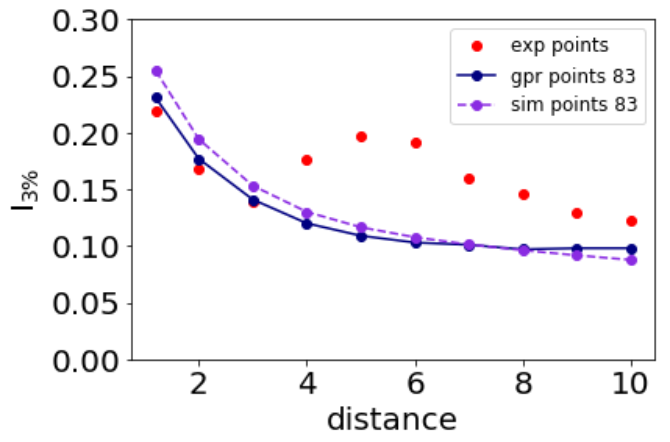
\includegraphics[width=7cm]{images/picGA_I3.png}
		%\caption{fig1}
	}
	\quad
	\subfigure[The performance of $I_{15{\%}}$.]{
		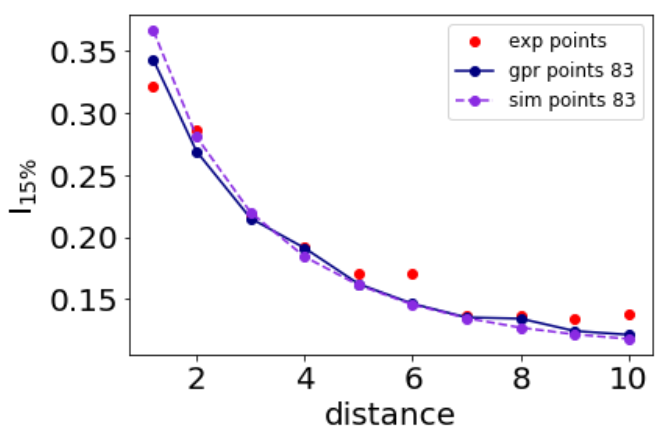
\includegraphics[width=7cm]{images/picGA_I15.png}
	}
	\quad
	\subfigure[The performance of $U_{3{\%}}$.]{
		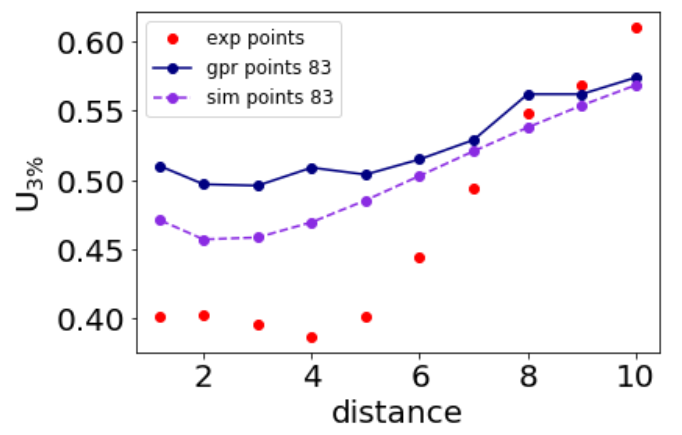
\includegraphics[width=7cm]{images/picGA_U3.png}
	}
	\quad
	\subfigure[The performance of $U_{15\%}$.]{
		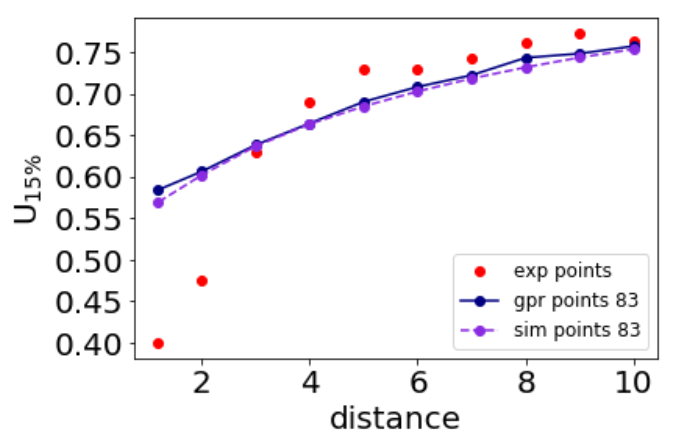
\includegraphics[width=7cm]{images/picGA_U15.png}
	}
	\caption{Comparison of physical experiments(red dots), GPR (blue line-dot curve), and simulation(purple dash-dot curve) in final${_3}$ via GA.}
	\label{fig:GA picture}
\end{figure}

PSO is operated by global and individual comparison. In our case, the initial particle population is set in 1000. The learning rate is [$c_{1}$,$c_{2}$]=[0.6, 0.5]. The stopping criteria of PSO is reach to maximum iteration 1000.

Table \ref{tab:PSO table} presents information about the performance of GPR and Particle Swarm Optimization (PSO). Because final error MAPE$_{sim/exp}$ of final${_1}$ is not within 23${\%}$, final${_1}$ should go to the second round of simulator. It turns out to be final${_2}$ with optimal fitting error MAPE$_{srgt/sim}$ (8.69${\%}$) and final error MAPE$_{sim/exp}$ (25.15${\%}$). There is a marginally increment in optimal fitting error MAPE$_{srgt/sim}$ up 0.03${\%}$ compared with final${_1}$, whereas final error MAPE$_{sim/exp}$ is in decline, dropping to 25.15${\%}$ not below to 23${\%}$. There is a need to go on the third round. Final${_3}$ turns out to be optimal fitting error MAPE$_{srgt/sim}$ (6.22${\%}$) and final error MAPE$_{sim/exp}$ (21.42${\%}$), as they all below to the standard of 10${\%}$ and 23${\%}$, individually. It is the end of the estimation of GPR and PSO's parameters.

During these three times of experiment, it shows that the gap of fitting error MAPE$_{srgt/sim}$ and optimal fitting error MAPE$_{srgt/sim}$ are within 5${\%}$. While GPR is trained in historical data, it can gradually catch the trend of the simulator with estimation more and more accurate. Likewise, there is a narrow gap between predicted error MAPE$_{srgt/exp}$ and final error MAPE$_{sim/exp}$ because GPR can fit the simulation data precisely.

$\beta_{p}$, $\beta_{d}$, $C_{\epsilon4}$, $C_{\epsilon5}$ are prone to hit their upper bounds or lower bounds bu using PSO. After three times of estimation, we get $\beta_{p}$ and $C_{\epsilon5}$ laying in their lower bounds. The remaining ones are between 0.1 and 4. In contrast, there is no parameter hitting the upper bound or the lower bound in GA. Overall, neither the combination of parameters in GA nor the parameters in PSO are not the same. 

\begin{minipage}{\linewidth}
	\centering
	\renewcommand\arraystretch{0.7}
	~\\
	\captionof{table}{GPR-surrogate and PSO estimated parameters and corresponding performances} \label{tab:PSO table} 
	\begin{tabular}{cccc}
		\hline
		{\small } &{\small } &{GPR and PSO}\\
		\hline
		{\small Parameter} & {\small Final${_1}$} & {\small Final${_2}$} & {\small Final${_3}$}\\
		\hline
		{$\beta_{p}$} & 0.9254 & 0.1 & 0.1 \\
		{$\beta_{d}$} & 0.1 & 3.843 & 2.25 \\
		{$C_{\epsilon4}$} & 1 & 0.4581 & 0.7 \\
		{$C_{\epsilon5}$} & 0.1 & 0.127 & 0.1\\
		\hline
		{Fitting Error MAPE$_{srgt/sim}$} & 5${\%}$ & 5.03${\%}$ & 6.25${\%}$\\
		{Predicted Error MAPE$_{srgt/exp}$} & 30.65${\%}$ & 25.15${\%}$ & 20.16${\%}$\\
		{Optimal Fitting Error MAPE$_{srgt/sim}$} & 8.66${\%}$ & 8.69${\%}$ & 6.22${\%}$\\
		{Final Error MAPE$_{sim/exp}$} & 28.28${\%}$ & 25.15${\%}$ & 21.42${\%}$\\
		\hline
	\end{tabular}
\end{minipage}

\begin{figure}[htbp]
	\centering
	\subfigure[The performance of $I_{3{\%}}$.]{
		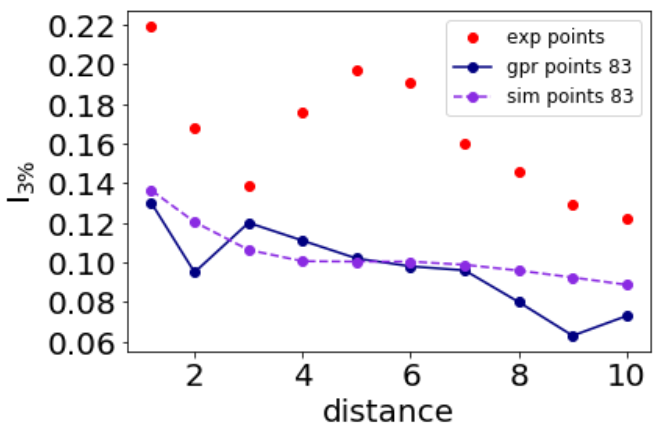
\includegraphics[width=7cm]{images/picPSO_I3.png}
		%\caption{fig1}
	}
	\quad
	\subfigure[The performance of $I_{15{\%}}$.]{
		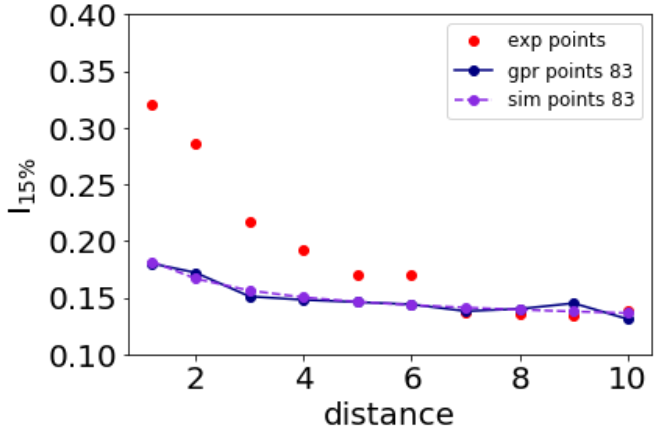
\includegraphics[width=7cm]{images/picPSO_I15.png}
	}
	\quad
	\subfigure[The performance of $U_{3{\%}}$.]{
		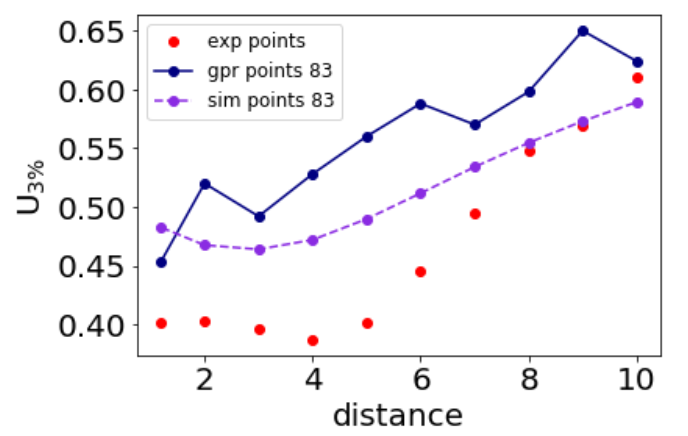
\includegraphics[width=7cm]{images/picPSO_U3.png}
	}
	\quad
	\subfigure[The performance of $U_{15\%}$.]{
		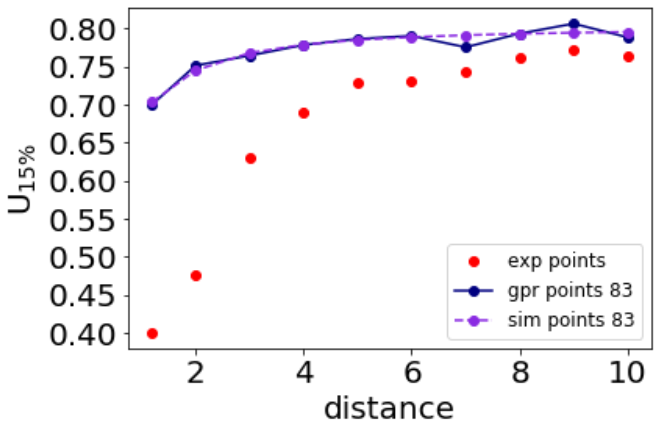
\includegraphics[width=7cm]{images/picPSO_U15.png}
	}
	\caption{Comparison of physical experiments(red dots), GPR (blue line-dot curve), and simulation(purple dash-dot curve) in final${_3}$ via PSO.}
	\label{fig:PSO picture}
\end{figure}
~\\

\chapter{Conclusion}

This paper emphasizes on data preprocessing, the building of surrogate model and metaheuristics instead of exploring the physical principle of marine turbine. As our surrogate model is built from historical simulation data which is not close to physical experiment, we apply some data preprocessing to increase accuracy of surrogate model's prediction. Then, we illustrate the use of the Gaussian surrogate model and metaheuristics to determine a set of unknown physical parameters based on historical information and define evaluative criteria to explain the model's accuracy. Our surrogate models are evaluated by MAPE, which compares the surrogate model's predictions with the physical experiment. By minimizing these surrogates' MAPE, the values of the unknown physical parameters are estimated via metaheuristics like GA and PSO. If the MAPE of optimal solution fitting error or final error are not within the range, we will add the optimal solution which is generated by each run of the simulation. Finally, we get final error MAPE$_{sim/exp}$ 14.23${\%}$ via the third round of GA. The application of the surrogate methodology to the marine turbine problem provides the advantage of neglecting all the physical information about the system when building a model. This method also shows the potential of reducing the burden to solve marine turbine problems when computationally-expensive numerical simulations are required. 

In our marine turbine's problem, we find twenty-six surrogate models and use the best of them to build the model, but we haven't tried Gaussian Mixture Model as a surrogate model. Although we used K-means clustering to retrieve the points which is close to physical experiments, we haven't used Density Base Scan to select the best dataset. We suggest that the followers can go deep into these aspects in the future. 
